\documentclass{article}%
\usepackage[T1]{fontenc}%
\usepackage[utf8]{inputenc}%
\usepackage{lmodern}%
\usepackage{textcomp}%
\usepackage{lastpage}%
%
\usepackage{amsmath}%
\usepackage{amssymb}%
\usepackage{amsfonts}%
\usepackage{graphicx}%
\usepackage{hyperref}%
\usepackage{tikz}%
\usepackage{pgfplots}%
\usetikzlibrary{math}%
\title{ITA 2026 - Matemática\thanks{This exam was solved and automatically generated with gpt-resolve: \url{https://github.com/lgabs/gpt-resolve}}}%
\author{claude{-}haiku{-}5{-}5 (solver) + claude{-}haiku{-}5{-}5 (judge)}%
\date{November 10, 2026}%
%
\begin{document}%
\normalsize%
\maketitle%
\section*{Questão 1}

\section*{Solução}

\textbf{1. Vértices do octaedro.} Um octaedro regular é a união de duas pirâmides regulares de base quadrada $ABCD$, de centro $M$, com ápices $P$ e $Q$ em lados opostos do plano da base e $PM=QM$. Logo $M$ é ponto médio de $\overline{AC}$, de $\overline{BD}$ e de $\overline{PQ}$: vértices opostos são simétricos em relação ao centro do sólido. Como o centro é a origem $O$, os seis vértices formam três pares antípodas $\{V,-V\}$.

Os pontos dados são $A_1=(5,0,0)$, $A_2=(0,5,0)$, $A_3=(0,0,5)$. Nenhum par deles é antípoda: o antípoda de $A_1$ é $(-5,0,0)$, que não coincide com $A_2$ nem com $A_3$; o mesmo vale para os demais. Logo $A_1,A_2,A_3$ estão em três pares distintos, pois dois deles no mesmo par seriam antípodas. Como há exatamente três pares, cada par contém exatamente um deles (se algum par não contivesse nenhum, os três pontos estariam em dois pares, e algum par teria dois, o que é impossível). Portanto os vértices são
\[
\pm 5e_1,\qquad \pm 5e_2,\qquad \pm 5e_3,\qquad e_1=(1,0,0),\ e_2=(0,1,0),\ e_3=(0,0,1).
\]
Conferência: a aresta $\overline{(5,0,0)(0,5,0)}$ mede $\sqrt{50}=5\sqrt2$, e a diagonal $\overline{(5,0,0)(-5,0,0)}$ mede $10=\sqrt2\cdot 5\sqrt2$, como num octaedro regular.

\textbf{2. O sólido como desigualdade.} Sejam $g(x,y,z)=|x|+|y|+|z|$ e $S=\{(x,y,z)\in\mathbb{R}^3 : g(x,y,z)\le 5\}$. O sólido é o fecho convexo $K=\operatorname{conv}\{\pm5e_1,\pm5e_2,\pm5e_3\}$. Provemos $K=S$.
\begin{itemize}
\item[(i)] $K\subseteq S$. Seja $P=\sum_j\lambda_jV_j$, com vértices $V_j$, $\lambda_j\ge 0$ e $\sum_j\lambda_j=1$. Pela desigualdade triangular, $|P_i|=\bigl|\sum_j\lambda_j(V_j)_i\bigr|\le\sum_j\lambda_j\,|(V_j)_i|$ para cada coordenada $i$. Somando em $i$: $g(P)\le\sum_j\lambda_j\,g(V_j)=\sum_j\lambda_j\cdot 5=5$, pois $g(\pm5e_i)=5$.
\item[(ii)] $S\subseteq K$. Seja $P=(x_1,x_2,x_3)$ com $g(P)\le 5$. Tome $s_i=1$ se $x_i\ge 0$ e $s_i=-1$ se $x_i<0$, de modo que $s_i|x_i|=x_i$. Então
\[
P=\sum_{i=1}^{3}\frac{|x_i|}{5}\,(5s_ie_i)+\frac{5-g(P)}{10}\,(5e_1)+\frac{5-g(P)}{10}\,(-5e_1).
\]
Verificação: a $i$-ésima coordenada da soma é $\frac{|x_i|}{5}\cdot 5s_i=s_i|x_i|=x_i$, e os dois últimos termos se cancelam. Os pesos são não negativos, pois $g(P)\le 5$, e somam $\frac{g(P)}{5}+2\cdot\frac{5-g(P)}{10}=1$. Logo $P\in K$.
\end{itemize}
Portanto $K=S$.

\textbf{3. Interior e superfície.} A função $g$ é contínua.
\begin{itemize}
\item Se $g(P)<5$, o conjunto $\{g<5\}$ é aberto (imagem inversa de aberto por função contínua) e está contido em $S$. Logo $P$ é ponto interior.
\item Se $g(P)=5$, então $P\in S$, mas $P$ não é interior. Seja $u=(s_1,s_2,s_3)$ com $s_i$ como acima e $\varepsilon>0$. Em cada coordenada, $|x_i+\varepsilon s_i|=|x_i|+\varepsilon$: se $x_i\ge 0$, então $x_i+\varepsilon>0$; se $x_i<0$, então $x_i-\varepsilon<0$. Logo $g(P+\varepsilon u)=5+3\varepsilon>5$, ou seja, $P+\varepsilon u\notin S$, e $P+\varepsilon u\to P$ quando $\varepsilon\to 0$. Assim $P$ está na superfície.
\end{itemize}
Portanto, interior $=\{g<5\}$ e superfície $=\{g=5\}$. Seja $N_k=\#\{(x,y,z)\in\mathbb{Z}^3 : g(x,y,z)=k\}$. Como $g$ é inteiro em $\mathbb{Z}^3$,
\[
\text{interior}=\sum_{k=0}^{4}N_k,\qquad \text{superfície}=N_5,\qquad \text{total}=\sum_{k=0}^{5}N_k.
\]

\textbf{4. Cálculo de $N_k$.} Seja $M(m)=\#\{(x,y)\in\mathbb{Z}^2 : |x|+|y|=m\}$.
\begin{itemize}
\item $M(0)=1$, pois só $(0,0)$ serve.
\item Para $m\ge 1$: se $|x|=m$, então $y=0$, o que dá $2$ pontos. Se $|x|\le m-1$ (há $2m-1$ valores de $x$), então $|y|=m-|x|\ge 1$ tem exatamente $2$ soluções em $y$. Logo $M(m)=2+2(2m-1)=4m$.
\end{itemize}
Fixe $z=t$ com $|t|\le k$. A condição $g=k$ vira $|x|+|y|=k-|t|$, com $M(k-|t|)$ soluções. O termo $t=0$ aparece uma vez, e cada $j=|t|\in\{1,\dots,k\}$ aparece para $t=\pm j$. Logo
\[
N_k=\sum_{t=-k}^{k}M(k-|t|)=M(k)+2\sum_{r=0}^{k-1}M(r).
\]
Para $k\ge 1$, $\sum_{r=0}^{k-1}M(r)=M(0)+\sum_{r=1}^{k-1}4r=1+2k(k-1)$. Então
\[
N_k=4k+2\bigl(1+2k(k-1)\bigr)=4k+2+4k^2-4k=4k^2+2,
\]
e $N_0=1$. Assim:
\[
N_1=4\cdot 1+2=6,\quad N_2=4\cdot 4+2=18,\quad N_3=4\cdot 9+2=38,\quad N_4=4\cdot 16+2=66,\quad N_5=4\cdot 25+2=102.
\]
Logo, interior: $1+6+18+38+66=129$; superfície: $N_5=102$; total: $129+102=231$.

\textbf{5. Conferência por tipos de coordenadas.} Para cada $k$, uma terna de módulos $(|x|,|y|,|z|)$ com soma $k$ corresponde a $(\text{número de permutações distintas})\cdot 2^{(\text{número de entradas não nulas})}$ pontos, pois cada entrada não nula admite sinal $\pm$. Usando todas as partições de $k$ em no máximo $3$ partes:
\begin{itemize}
\item $k=1$: $(1,0,0)$ dá $3\cdot 2=6$.
\item $k=2$: $(2,0,0)$ dá $3\cdot 2=6$; $(1,1,0)$ dá $3\cdot 4=12$. Total $18$.
\item $k=3$: $(3,0,0)$ dá $6$; $(2,1,0)$ dá $6\cdot 4=24$; $(1,1,1)$ dá $8$. Total $6+24+8=38$.
\item $k=4$: $(4,0,0)$ dá $6$; $(3,1,0)$ dá $24$; $(2,2,0)$ dá $3\cdot 4=12$; $(2,1,1)$ dá $3\cdot 8=24$. Total $6+24+12+24=66$.
\item $k=5$: $(5,0,0)$ dá $6$; $(4,1,0)$ dá $24$; $(3,2,0)$ dá $24$; $(3,1,1)$ dá $3\cdot 8=24$; $(2,2,1)$ dá $3\cdot 8=24$. Total $6+24+24+24+24=102$.
\end{itemize}
Os totais coincidem com $N_k$.

\textbf{6. Fórmula geral e casos particulares.} Seja $N(n)=\#\{(x,y,z)\in\mathbb{Z}^3 : g\le n\}$. Então
\[
N(n)=1+\sum_{k=1}^{n}(4k^2+2)=1+\frac{2n(n+1)(2n+1)}{3}+2n=\frac{(2n+1)(2n^2+2n+3)}{3},
\]
pois, multiplicando por $3$, $3+2n(n+1)(2n+1)+6n=4n^3+6n^2+8n+3=(2n+1)(2n^2+2n+3)$.
Casos particulares: $N(0)=\frac{1\cdot 3}{3}=1$ (só a origem); $N(1)=\frac{3\cdot 7}{3}=7$ (origem e os 6 vértices); $N(2)=\frac{5\cdot 15}{3}=25=1+6+18$, conferido à mão pelas contagens acima; e $N(5)=\frac{11\cdot 63}{3}=\frac{693}{3}=231$, com $2\cdot 25+2\cdot 5+3=63$.

\textbf{7. Unidades e ordem de grandeza.} A resposta é uma contagem, portanto adimensional. O sólido é a união de duas pirâmides de base quadrada com diagonal $10$ (área $\frac{10\cdot 10}{2}=50$) e altura $5$, de volume $V=2\cdot\frac13\cdot 50\cdot 5=\frac{500}{3}\approx 166{,}7$. A contagem $231$ tem a mesma ordem de grandeza de $V$, e a diferença $\approx 64$ é plausível como contribuição dos pontos de fronteira. Isto é uma checagem de plausibilidade, não uma prova.

Portanto há $231$ pontos com todas as coordenadas inteiras no interior ou na superfície do octaedro: $129$ no interior e $102$ na superfície.

ANSWER: 231 pontos (129 no interior e 102 na superfície)%
\newpage%
\section*{Questão 2}

\section*{Solução}

\textbf{1. Forma geral de $A^n$.} Afirmamos que, para todo $n\in\mathbb{N}$,
\begin{equation*}
A^n=\begin{bmatrix}1 & n & a_n\\ 0 & 1 & n\\ 0 & 0 & 1\end{bmatrix},\qquad a_n=\frac{n(n+3)}{2}.
\end{equation*}

Demonstração por indução em $n$.

\emph{Base ($n=1$):} $a_1=\frac{1\cdot 4}{2}=2$, e a matriz acima é exatamente $A$.

\emph{Passo indutivo:} supondo a afirmação válida para $n$, temos $A^{n+1}=A^n\cdot A$. A entrada $(i,j)$ de $A^{n+1}$ é o produto da linha $i$ de $A^n$ pela coluna $j$ de $A$. As colunas de $A$ são $(1,0,0)^T$, $(1,1,0)^T$ e $(2,1,1)^T$.

\begin{itemize}
\item Linha 1 de $A^n$: $(1,\ n,\ a_n)$. Com as colunas de $A$ obtemos $1$, $1+n$ e $2+n+a_n$.
\item Linha 2 de $A^n$: $(0,\ 1,\ n)$. Obtemos $0$, $1$ e $1+n$.
\item Linha 3 de $A^n$: $(0,\ 0,\ 1)$. Obtemos $0$, $0$ e $1$.
\end{itemize}

Portanto
\begin{equation*}
A^{n+1}=\begin{bmatrix}1 & n+1 & a_n+n+2\\ 0 & 1 & n+1\\ 0 & 0 & 1\end{bmatrix}.
\end{equation*}
Resta verificar que $a_n+n+2=a_{n+1}$:
\begin{equation*}
a_n+n+2=\frac{n^2+3n+2n+4}{2}=\frac{(n+1)(n+4)}{2}=\frac{(n+1)\big((n+1)+3\big)}{2}=a_{n+1}.
\end{equation*}
As entradas $(1,2)$ e $(2,3)$ de $A^{n+1}$ são $n+1$, logo a forma vale para $n+1$. Isso completa a indução.

\textbf{2. Entrada pedida.} Pelo item 1, a entrada na primeira linha e terceira coluna de $A^n$ é
\begin{equation*}
a_n=\frac{n(n+3)}{2}, \qquad n\in\mathbb{N}.
\end{equation*}

\textbf{3. Resolução da desigualdade.} Queremos o menor $n\in\mathbb{N}$ com $a_n>119$. Multiplicando por $2>0$ e usando $(n-14)(n+17)=n^2+3n-238$:
\begin{equation*}
a_n>119 \iff n^2+3n-238>0 \iff (n-14)(n+17)>0.
\end{equation*}
Para $n\in\mathbb{N}$ temos $n+17>0$, logo a condição se reduz a $n-14>0$, isto é, $n>14$. O menor natural com essa propriedade é $n=15$.

\textbf{Conferência.}
\begin{itemize}
\item Caso limite: $a_{14}=\frac{14\cdot 17}{2}=119$. Como a desigualdade é estrita, $n=14$ não serve.
\item $a_{15}=\frac{15\cdot 18}{2}=135>119$.
\item Pela recorrência $a_{n+1}-a_n=n+2$: $a_{13}=104$, $a_{14}=119$, $a_{15}=135$ (diferenças $15$ e $16$, como previsto).
\item Cálculo direto: $(A^2)_{13}=1\cdot 2+1\cdot 1+2\cdot 1=5=a_2$.
\item Ordem de grandeza: $a_n\approx n^2/2$, e $n^2\approx 238$ leva a $n\approx 15$, coerente com o resultado.
\end{itemize}

ANSWER: $n = 15$ (com $a_{15}=135$; para $n=14$ a entrada vale exatamente $119$, o que não satisfaz "maior que $119$")%
\newpage%
\section*{Questão 3}

\section*{Solução}

Notação: $r:\ x-2y+2=0$ e $s:\ x+2y-8=0$. A circunferência dada, $\Gamma$, tem centro $I=\left(\tfrac12,\tfrac52\right)$ e raio $\rho=\tfrac{\sqrt5}{2}$, pois $\rho^2=\tfrac54$.

\textbf{Passo 1 (ponto X).} Em $r$, $x=2y-2$. Substituindo em $s$: $(2y-2)+2y=8$, logo $y=\tfrac52$ e $x=3$. Assim $X=\left(3,\tfrac52\right)$. Os coeficientes angulares são $\tfrac12$ e $-\tfrac12$, logo as retas não são paralelas e $X$ é o único ponto comum.

\textbf{Passo 2 (X é o centro do paralelogramo).} Seja $O$ a interseção das diagonais. Em um paralelogramo, $O$ é ponto médio de $\overline{AC}$ e de $\overline{BD}$. Cada diagonal está contida em uma das retas $r$, $s$, e essas retas são distintas (caso contrário os quatro vértices seriam colineares). Como $C\in r$ ($2\cdot5-8=2$) e $C\notin s$ ($8+2\cdot5=18\neq8$), a reta que contém $\overline{AC}$ é $r$; logo $\overline{BD}\subset s$. Então $O\in r\cap s=\{X\}$, ou seja, $O=X$. Em particular, $X$ é ponto médio de $\overline{AC}$ e de $\overline{BD}$, e $B\in s$.

\textbf{Passo 3 (vértice A).} Como $X$ é ponto médio de $\overline{AC}$:
\[
A=2X-C=(6-8,\;5-5)=(-2,0).
\]
Conferência: $2\cdot0-(-2)=2$, logo $A\in r$.

\textbf{Passo 4 ($r$ e $s$ tangenciam $\Gamma$).}
\[
d(I,r)=\frac{\left|\tfrac12-5+2\right|}{\sqrt5}=\frac{\tfrac52}{\sqrt5}=\frac{\sqrt5}{2}=\rho,
\qquad
d(I,s)=\frac{\left|\tfrac12+5-8\right|}{\sqrt5}=\frac{\sqrt5}{2}=\rho.
\]
Como $X,A\in r$ e $X,B\in s$, as retas $r$ e $s$ são as retas dos lados $\overline{XA}$ e $\overline{XB}$ do triângulo $ABX$. Se $\Gamma$ é a inscrita, ela também tangencia a reta $AB$.

\textbf{Passo 5 (reta AB e vértice B).} O ponto $A$ é exterior a $\Gamma$, pois $AI^2=\tfrac{25}{2}>\tfrac54$. Por $A$ passam então exatamente duas tangentes a $\Gamma$, e uma delas é $r$. Como $B\in s$ e $B\neq X$ (triângulo não degenerado), $B\notin r$. Logo $AB$ é a outra tangente. A reta vertical $x=-2$ está a distância $\tfrac52\neq\rho$ de $I$, então não é tangente. Escrevendo a reta por $A$ como $mx-y+2m=0$:
\[
d(I,AB)=\frac{\left|\tfrac m2-\tfrac52+2m\right|}{\sqrt{m^2+1}}=\frac{\tfrac52\,|m-1|}{\sqrt{m^2+1}}=\frac{\sqrt5}{2}.
\]
Então $5|m-1|=\sqrt5\,\sqrt{m^2+1}$. Elevando ao quadrado: $25(m-1)^2=5(m^2+1)$, ou seja, $2m^2-5m+2=0$, isto é, $(2m-1)(m-2)=0$. A raiz $m=\tfrac12$ corresponde à reta $r$ (que passa por $A$). Logo $AB:\ y=2x+4$, isto é, $2x-y+4=0$.

Agora $B=AB\cap s$: substituindo $y=2x+4$ em $x+2y=8$ obtemos $x+4x+8=8$, logo $x=0$ e $y=4$:
\[
B=(0,4).
\]
Conferência: $0+2\cdot4=8$, logo $B\in s$.

\textbf{Passo 6 (verificação de que $\Gamma$ é a inscrita).} O triângulo é não degenerado: $\det(B-A,\,X-A)=\det\begin{pmatrix}2&5\\4&\tfrac52\end{pmatrix}=5-20=-15\neq0$. Os três lados estão a distância $\rho$ de $I$: $r$ e $s$ pelo Passo 4, e
\[
d(I,AB)=\frac{\left|2\cdot\tfrac12-\tfrac52+4\right|}{\sqrt5}=\frac{\tfrac52}{\sqrt5}=\frac{\sqrt5}{2}=\rho.
\]
Para que $I$ seja interior, ele deve estar do mesmo lado de cada reta que o vértice oposto. Com $f_r=x-2y+2$, $f_s=x+2y-8$ e $f_{AB}=2x-y+4$:
\begin{itemize}
\item $f_r(I)=-\tfrac52$ e $f_r(B)=-6$: mesmo sinal;
\item $f_s(I)=-\tfrac52$ e $f_s(A)=-10$: mesmo sinal;
\item $f_{AB}(I)=\tfrac52$ e $f_{AB}(X)=\tfrac{15}{2}$: mesmo sinal.
\end{itemize}
Logo $I$ é interior a $ABX$ e equidistante dos três lados, isto é, é o incentro, e $\rho$ é o inraio. Portanto $\Gamma$ é a circunferência inscrita em $ABX$, como dado. Como $B$ foi forçado pela condição de tangência, esta é a única escolha possível.

\textbf{Passo 7 (vértice D).} Como $X$ é ponto médio de $\overline{BD}$:
\[
D=2X-B=(6-0,\;5-4)=(6,1),
\]
com $6+2\cdot1=8$, logo $D\in s$. Conferências: $A+C=(6,5)=B+D$ e $\overrightarrow{AB}=(2,4)=\overrightarrow{DC}$, portanto $ABCD$ é paralelogramo.

Observação: trocar os rótulos $B$ e $D$ daria o mesmo conjunto de vértices e a mesma área, mas $\Gamma$ não seria inscrita no triângulo com vértice $(6,1)$. A distância de $I$ à reta por $A$ e $(6,1)$ é $\tfrac{35}{2\sqrt{65}}\approx 2{,}17$, diferente de $\rho\approx 1{,}12$.

\textbf{Passo 8 (área).} Com $\overrightarrow{AB}=(2,4)$ e $\overrightarrow{AD}=(8,1)$, a área do paralelogramo é o módulo do determinante dos lados adjacentes:
\[
S_{ABCD}=\left|\det\begin{pmatrix}2&8\\4&1\end{pmatrix}\right|=|2\cdot1-8\cdot4|=|-30|=30.
\]

\textbf{Verificações independentes.}
\begin{itemize}
\item Pelas diagonais: $\overrightarrow{AC}=\overrightarrow{AB}+\overrightarrow{AD}$ e $\overrightarrow{BD}=\overrightarrow{AD}-\overrightarrow{AB}$, logo $\overrightarrow{AC}\times\overrightarrow{BD}=2\,(\overrightarrow{AB}\times\overrightarrow{AD})$ e $S=\tfrac12\left|\overrightarrow{AC}\times\overrightarrow{BD}\right|$. Com $\overrightarrow{AC}=(10,5)$ e $\overrightarrow{BD}=(6,-3)$: $\tfrac12\left|10\cdot(-3)-5\cdot6\right|=\tfrac12\cdot60=30$.
\item Pelos triângulos: como $X$ é ponto médio das duas diagonais, os quatro triângulos $ABX$, $BCX$, $CDX$, $DAX$ têm a mesma área. Logo $S=4\,[ABX]=4\cdot\tfrac12\cdot15=30$.
\item Ordem de grandeza: $|AC|=5\sqrt5\approx11{,}18$ e $|BD|=3\sqrt5\approx6{,}71$, com $|AC|\,|BD|=75$. Como $S\le\tfrac12|AC|\,|BD|=37{,}5$, o valor 30 é plausível. Exatamente, $\cos\varphi=\dfrac{10\cdot6+5\cdot(-3)}{75}=\dfrac35$ e $\operatorname{sen}\varphi=\dfrac45$, donde $S=\tfrac12\cdot75\cdot\tfrac45=30$.
\end{itemize}

Unidades: as coordenadas estão na mesma unidade de comprimento, logo a área está em unidades de área.

Vértices: $A(-2,0)$, $B(0,4)$, $C(8,5)$, $D(6,1)$.

ANSWER: 30 unidades de área%
\newpage%
\section*{Questão 4}

\section*{Solução}

\textbf{Notação e interpretação.} Seja $\alpha>0$ o raio do disco central, em unidades de comprimento. Os 33 círculos (contando o central) são concêntricos, com raios $R_k=\alpha+k$, para $k=0,1,\ldots,32$. Seja $D_0$ o disco de raio $R_0=\alpha$ e, para $1\leq k\leq 32$, seja $A_k$ o anel compreendido entre os círculos de raios $R_{k-1}$ e $R_k$.

\textbf{Cores.} O disco $D_0$ é vermelho e as cores alternam de anel em anel. Assim, $A_1$ é branco, $A_2$ é vermelho, $A_3$ é branco, e, em geral, $A_k$ é vermelho se, e somente se, $k$ é par. Os anéis vermelhos são $A_{2j}$ com $j=1,2,\ldots,16$ (o mais externo é $A_{32}$), e os brancos são $A_{2j-1}$ com $j=1,\ldots,16$.

\textbf{Área de um anel.} Os círculos são concêntricos, logo $A_k$ é a diferença entre os discos de raios $R_k$ e $R_{k-1}$. Pela aditividade da área,
\[
[A_k]=\pi R_k^2-\pi R_{k-1}^2=\pi\big[(\alpha+k)^2-(\alpha+k-1)^2\big].
\]
Pela identidade $x^2-(x-1)^2=2x-1$, com $x=\alpha+k$, obtemos
\[
[A_k]=\pi\,(2\alpha+2k-1).
\]
Por exemplo, $[A_1]=\pi\big[(\alpha+1)^2-\alpha^2\big]=\pi(2\alpha+1)$.

\textbf{Área vermelha.} A região vermelha é a reunião do disco $D_0$ com os anéis $A_{2j}$, $j=1,\ldots,16$. Como para $k=2j$ temos $2\alpha+2k-1=2\alpha+4j-1$,
\[
S_V=\pi\alpha^2+\sum_{j=1}^{16}\pi\,(2\alpha+4j-1).
\]
Na soma, o termo $2\alpha-1$ é somado 16 vezes e $\sum_{j=1}^{16} j=\dfrac{16\cdot 17}{2}=136$. Logo
\[
\sum_{j=1}^{16}(2\alpha+4j-1)=16\cdot 2\alpha+4\cdot 136-16=32\alpha+544-16=32\alpha+528.
\]
Portanto
\[
S_V=\pi\,(\alpha^2+32\alpha+528).
\]

\textbf{Verificação.} Os anéis brancos são $A_{2j-1}$, com $[A_{2j-1}]=\pi(2\alpha+4j-3)$. Assim
\[
S_B=\sum_{j=1}^{16}\pi(2\alpha+4j-3)=\pi(32\alpha+544-48)=\pi(32\alpha+496).
\]
A soma das áreas vermelha e branca deve ser a área do círculo externo, de raio $\alpha+32$:
\[
S_V+S_B=\pi(\alpha^2+64\alpha+1024)=\pi(\alpha+32)^2.
\]
Isso confirma o resultado.

\textbf{Casos particulares e ordem de grandeza.}
\begin{itemize}
\item Para $\alpha=1$: $S_V=561\pi$, $S_B=528\pi$ e a área total é $1089\pi=33^2\pi$. Também $[A_2]=\pi(3^2-2^2)=5\pi=\pi(2\cdot 1+4-1)$, de acordo com a fórmula.
\item A diferença $S_V-S_B=\pi(\alpha^2+32)$ é coerente: cada par $(A_{2j},A_{2j-1})$ difere em $2\pi$, e são 16 pares, o que dá $32\pi$. O disco central acrescenta $\pi\alpha^2$.
\item Para $\alpha$ grande, $S_V\approx\pi\alpha^2$, pois o disco central domina. Além disso, $S_B\approx 32\pi\alpha$, já que cada anel de largura 1 tem área $\approx 2\pi\alpha$ e há 16 anéis brancos.
\end{itemize}

Como a questão pede uma expressão em função de $\alpha$, a resposta final é a área vermelha $S_V(\alpha)$ indicada abaixo, em unidades de área.

ANSWER: $S_{\text{vermelho}}(\alpha)=\pi\,(\alpha^2+32\alpha+528)$ unidades de área%
\newpage%
\section*{Questão 5}

\section*{Solução}

\textbf{Notação.} Sejam $r$ o raio das esferas menores, $R$ o raio da esfera maior, $O$ o centro da esfera maior, $C_1,C_2,C_3,C_4$ os centros das esferas menores e $a$ a aresta do tetraedro regular $C_1C_2C_3C_4$.

\textbf{Passo 1 (aresta em função de $r$).} Sejam $i\neq j$. Se as esferas $i$ e $j$ fossem tangentes internamente, a distância entre seus centros seria $|r-r|=0$, isto é, as esferas coincidiriam, o que é absurdo, pois são quatro esferas distintas. Logo a tangência é exterior, e a distância entre os centros é a soma dos raios:
\[
a = m(\overline{C_iC_j}) = r + r = 2r.
\]

\textbf{Passo 2 ($O$ é o circuncentro do tetraedro).} Cada esfera menor está contida na esfera maior e é tangente a ela, logo a tangência é interna. Em duas esferas tangentes internamente, o ponto de tangência, $O$ e o centro da esfera menor estão alinhados, e a distância entre os centros é a diferença dos raios. Portanto
\[
m(\overline{OC_i}) = R - r \qquad (i=1,2,3,4).
\]
Assim, $O$ é equidistante dos quatro vértices do tetraedro. Esse ponto é único: se $P$ também é equidistante de $C_1,\dots,C_4$, expandindo $|P-C_1|^2=|P-C_k|^2$ obtém-se
\[
2\,P\cdot(C_k-C_1)=|C_k|^2-|C_1|^2 \qquad (k=2,3,4),
\]
um sistema linear cuja matriz tem linhas $C_k-C_1$ linearmente independentes, pois os vértices não são coplanares. Logo a solução é única, e $O$ é o circuncentro do tetraedro.

\textbf{Passo 3 (circunraio do tetraedro regular).} Os vértices $V_1=(1,1,1)$, $V_2=(1,-1,-1)$, $V_3=(-1,1,-1)$ e $V_4=(-1,-1,1)$ formam um tetraedro regular: dois quaisquer deles diferem em duas coordenadas por $2$, logo a distância entre eles é $\sqrt{8}=2\sqrt{2}$. A média dos quatro vértices é $(0,0,0)$, e cada vértice está à distância $\sqrt{3}$ da origem. Pelo passo anterior (unicidade do equidistante), a origem é o circuncentro desse tetraedro, e como é também o baricentro, o circuncentro coincide com o baricentro. Multiplicando as coordenadas por $\lambda=\dfrac{a}{2\sqrt{2}}$, obtém-se um tetraedro regular de aresta $a$ com o mesmo centro e circunraio $\sqrt{3}\,\lambda$. Como dois tetraedros regulares de mesma aresta são congruentes, o centro $O$ é o baricentro do tetraedro $C_1C_2C_3C_4$, e
\[
d = m(\overline{OC_i}) = \sqrt{3}\cdot\frac{a}{2\sqrt{2}} = \frac{a\sqrt{6}}{4}.
\]

\textbf{Passo 4 (raios).} Com $a=2r$ do Passo 1,
\[
d = \frac{2r\sqrt{6}}{4} = \frac{r\sqrt{6}}{2}.
\]
Como $m(\overline{OC_i}) = d = R - r$, temos $R = d + r$, logo
\[
R = \frac{r\sqrt{6}}{2} + r = \frac{(2+\sqrt{6})\,r}{2}, \qquad \frac{R}{r}=\frac{2+\sqrt{6}}{2}\approx 2{,}22 > 1.
\]

\textbf{Passo 5 (razão pedida).} O volume de uma esfera de raio $t$ é $\frac{4}{3}\pi t^3$. Logo
\[
\frac{V_{\text{maior}}}{\sum V_{\text{menores}}}
= \frac{\frac{4}{3}\pi R^3}{4\cdot\frac{4}{3}\pi r^3}
= \frac{R^3}{4r^3}
= \frac{1}{4}\left(\frac{2+\sqrt{6}}{2}\right)^3.
\]
Desenvolvendo as potências:
\[
(2+\sqrt{6})^2 = 4+4\sqrt{6}+6 = 10+4\sqrt{6},
\]
\[
(2+\sqrt{6})^3 = (10+4\sqrt{6})(2+\sqrt{6}) = 20+10\sqrt{6}+8\sqrt{6}+24 = 44+18\sqrt{6}.
\]
Logo $\left(\dfrac{2+\sqrt{6}}{2}\right)^3=\dfrac{44+18\sqrt{6}}{8}=\dfrac{22+9\sqrt{6}}{4}$. Finalmente, dividindo por $4$:
\[
\frac{V_{\text{maior}}}{\sum V_{\text{menores}}}
= \frac{1}{4}\cdot\frac{22+9\sqrt{6}}{4}
= \frac{22+9\sqrt{6}}{16}\approx 2{,}75.
\]

\textbf{Verificação.}
\begin{itemize}
\item A razão é adimensional e não depende de $r$, como deve ocorrer num quociente de volumes semelhantes.
\item Ordem de grandeza: as esferas menores têm interiores disjuntos e estão contidas na maior, logo a soma de seus volumes não excede $V_{\text{maior}}$ e a razão é $\geq 1$. Obteve-se $2{,}75$, e as menores ocupam $1/2{,}75\approx 36\%$ do volume da maior, valor que coincide com $4(r/R)^3\approx 0{,}363$.
\item Conferência independente de $d$: a altura do tetraedro satisfaz $h^2 = a^2-\left(\frac{a\sqrt{3}}{3}\right)^2=\frac{2a^2}{3}$, logo $h=\frac{a\sqrt{6}}{3}$. O baricentro divide a altura na razão $3:1$ a partir do vértice, de modo que $d=\frac{3}{4}h=\frac{a\sqrt{6}}{4}$, o mesmo valor obtido.
\item Numérica com $r=1$: $a=2$, $d=\frac{\sqrt{6}}{2}\approx 1{,}2247$, $R\approx 2{,}2247$, $R^3/4\approx 2{,}7528$, que coincide com $\frac{22+9\sqrt{6}}{16}$.
\end{itemize}

ANSWER: $\dfrac{22+9\sqrt{6}}{16}\approx 2{,}75$%
\newpage%
\section*{Questão 6}

\section*{Solução}

\textbf{Convenções e enunciado.} Confere-se o enunciado com a página 7 da prova: $a_{ij}=0$ se $j\ge i$, $a_{ij}=\alpha_j^{\,i-j-1}$ se $j<i$; $b_{ij}=1$ se $j\ge i$ e $b_{ij}=0$ se $j<i$. Usa-se $\alpha^{0}=1$ para todo $\alpha\in\mathbb{R}$, inclusive $\alpha=0$, para que $A$ esteja bem definida (por exemplo, $a_{j+1,j}=\alpha_j^{0}=1$). Denotem-se por $c_k=\sum_{i=1}^{n}a_{ik}$ a soma da coluna $k$ de $A$ e por $\sigma_j=\sum_{i=1}^{n}(AB)_{ij}$ a soma da coluna $j$ de $AB$. A hipótese é
\[
(H)\qquad \sigma_j=n-j,\quad j=1,\dots,n.
\]

\textbf{Passo 1: estrutura de $A$ e $B$.}
\begin{itemize}
\item Como $a_{ij}=0$ sempre que $j\ge i$, a matriz $A$ é triangular inferior com diagonal nula. Em particular, para todo $i\le n$ vale $n\ge i$, logo $a_{in}=0$: a coluna $n$ de $A$ é nula e $c_n=0$.
\item $B$ é triangular superior com diagonal de uns, logo $\det B=1$.
\end{itemize}

\textbf{Passo 2: colunas de $AB$.} Como $b_{kj}=1$ exatamente quando $k\le j$,
\[
(AB)_{ij}=\sum_{k=1}^{n}a_{ik}\,b_{kj}=\sum_{k=1}^{j}a_{ik}.
\]
Somando sobre $i$ e trocando a ordem de somas finitas,
\[
\sigma_j=\sum_{k=1}^{j}c_k .
\]
Em particular, $\sigma_n=\sum_{k=1}^{n}c_k$ é a soma de todas as entradas de $A$.

\textbf{Passo 3: a hipótese é inconsistente para $n\ge 2$.} Pelo Passo 2, $\sigma_n-\sigma_{n-1}=c_n=0$ para todos os $\alpha_j$. Já $(H)$ com $j=n$ e $j=n-1$ exige $\sigma_n-\sigma_{n-1}=0-1=-1$. Logo, para $n\ge 2$, nenhuma escolha de $\alpha_1,\dots,\alpha_{n-1}\in\mathbb{R}$ satisfaz $(H)$. Para $n=1$, $A=(0)$, $AB=(0)$ e $(H)$ vale, pois $\sigma_1=0=n-1$.

Verificação direta com $n=3$, $\alpha_1=2$, $\alpha_2=3$ (aqui $a_{21}=\alpha_1^{0}=1$, $a_{31}=\alpha_1^{1}=2$, $a_{32}=\alpha_2^{0}=1$):
\[
A=\begin{pmatrix}0&0&0\\1&0&0\\2&1&0\end{pmatrix},\qquad
B=\begin{pmatrix}1&1&1\\0&1&1\\0&0&1\end{pmatrix},\qquad
AB=\begin{pmatrix}0&0&0\\1&1&1\\2&3&3\end{pmatrix}.
\]
As somas das colunas de $AB$ são $3,4,4$, enquanto $(H)$ exige $2,1,0$.

\textbf{Item (a).} Pelo teorema de Binet, $\det(AB)=\det A\cdot\det B$, válido para quaisquer matrizes quadradas de mesma ordem. Como a coluna $n$ de $A$ é nula, toda parcela da fórmula de Leibniz para $\det A$ contém uma entrada nula, logo $\det A=0$. Portanto
\[
\det(AB)=0\cdot 1=0
\]
para todo $n$ e todos os $\alpha_j$. Esta conclusão não usa $(H)$.

\textbf{Item (b).} Como $a_{ik}=0$ para $k\ge i$, tem-se $\sum_{k\le i}a_{ik}=\sum_{k=1}^{n}a_{ik}$. Logo
\[
\operatorname{tr}(AB)=\sum_{i=1}^{n}(AB)_{ii}=\sum_{i=1}^{n}\sum_{k=1}^{n}a_{ik}=\sum_{k=1}^{n}c_k=\sigma_n .
\]
Sem hipótese, o traço é a soma das entradas de $A$ e depende dos $\alpha_j$ (no exemplo acima vale $4$). A hipótese com $j=n$ fixa $\sigma_n=0$, logo o valor pedido é
\[
\operatorname{tr}(AB)=0 \quad\text{para todo } n,
\]
que não depende de $n$. Ressalva: pelo Passo 3, para $n\ge 2$ esse $0$ é o valor exigido por $(H)$, mas nenhum $\alpha_j$ satisfaz $(H)$; é um valor formal. Para $n=1$, a hipótese vale e $\operatorname{tr}(AB)=0$ de fato.

\textbf{Item (c).} Para $n=5$, $(H)$ exige $\sigma_4=1$ e $\sigma_5=0$, donde $\sigma_5-\sigma_4=-1$. Mas
\[
\sigma_5-\sigma_4=c_5=\sum_{i=1}^{5}a_{i5}=0,
\]
pois $a_{i5}=0$ para todo $i\le 5$. A contradição $0=-1$ não envolve $\alpha_1,\alpha_2,\alpha_3,\alpha_4$; $\alpha_4$ aparece em $A$ apenas em $a_{54}=\alpha_4^{0}=1$. Logo não existe $(\alpha_1,\alpha_2,\alpha_3,\alpha_4)\in\mathbb{R}^4$ satisfazendo a hipótese: o conjunto pedido é vazio.

\textbf{Observação (leitura alternativa, não é o enunciado impresso).} Se $b_{kj}=1$ para $j\le k$ e $b_{kj}=0$ para $j>k$, então $(AB)_{ij}=\sum_{k\ge j}a_{ik}$ e $\sigma_j=\sum_{k\ge j}c_k$. Nessa leitura:
\begin{itemize}
\item $AB$ é estritamente triangular inferior: se $j\ge i$, todo $k\ge j$ satisfaz $k\ge i$, logo $a_{ik}=0$ e $(AB)_{ij}=0$. Assim $\det(AB)=0$ e $\operatorname{tr}(AB)=0$ continuam valendo.
\item Como $c_n=0$, tem-se $\sigma_n=0$ automaticamente, e $\sigma_j-\sigma_{j+1}=c_j$. Logo $(H)$ equivale a $c_j=1$ para $j=1,\dots,n-1$.
\item Para $n=5$, $c_j=\sum_{i=j+1}^{5}\alpha_j^{\,i-j-1}$, ou seja, $c_1=1+\alpha_1+\alpha_1^2+\alpha_1^3$, $c_2=1+\alpha_2+\alpha_2^2$, $c_3=1+\alpha_3$, $c_4=1$ (com $0^0=1$).
\begin{itemize}
\item $c_1=1\iff\alpha_1(1+\alpha_1+\alpha_1^2)=0\iff\alpha_1=0$, pois $1+\alpha_1+\alpha_1^2=\left(\alpha_1+\tfrac{1}{2}\right)^2+\tfrac{3}{4}>0$ em $\mathbb{R}$.
\item $c_2=1\iff\alpha_2(\alpha_2+1)=0\iff\alpha_2\in\{0,-1\}$.
\item $c_3=1\iff\alpha_3=0$.
\item $c_4=1$ sempre, logo $\alpha_4$ é livre em $\mathbb{R}$.
\end{itemize}
\end{itemize}
Nessa leitura, o conjunto solução é $\{(0,0,0,t)\}\cup\{(0,-1,0,t)\}$ com $t\in\mathbb{R}$. A discrepância sugere um possível erro de digitação no enunciado; vale conferir o gabarito oficial com essa possibilidade em mente.

ANSWER: (a) $\det(AB)=0$ para todo $n$ e todos os $\alpha_j$; (b) $\operatorname{tr}(AB)=0$ para todo $n$ (valor exigido por $\sigma_n=0$, formal para $n\ge 2$); (c) conjunto vazio: não existem $\alpha_1,\alpha_2,\alpha_3,\alpha_4\in\mathbb{R}$ satisfazendo a hipótese.%
\newpage%
\section*{Questão 7}

\section*{Solução}

\textbf{Passo 1 (forma de $p$).} O divisor $x^3-x+4$ é mônico e tem coeficientes reais, logo a divisão euclidiana em $\mathbb{R}[x]$ existe e é única: há quociente $q(x)$ e resto $r(x)$ em $\mathbb{R}[x]$ tais que
\[
p(x)=(x^3-x+4)\,q(x)+r(x), \qquad \operatorname{gr} r<3 .
\]
Aqui $r(x)=9x^2-4x+7$. Como $\operatorname{gr} p=4$ e $\operatorname{gr}(x^3-x+4)=3$, o quociente tem grau $1$: $q(x)=ax+b$, com $a,b\in\mathbb{R}$ e $a\neq 0$.

\textbf{Passo 2 (expansão).} Como $(x^3-x+4)(ax+b)=ax^4+bx^3-ax^2+(4a-b)x+4b$, temos
\begin{align*}
p(x)&=(x^3-x+4)(ax+b)+9x^2-4x+7\\
&=ax^4+bx^3+(9-a)x^2+(4a-b-4)x+(4b+7).
\end{align*}

\textbf{Passo 3 (relações de Girard).} Para $p(x)=c_4x^4+c_3x^3+c_2x^2+c_1x+c_0$ com $c_4\neq 0$, valem $\sum x_k=-\dfrac{c_3}{c_4}$ e $\prod x_k=\dfrac{c_0}{c_4}$; no produto o sinal é $(-1)^4=+1$. Com $c_4=a$, $c_3=b$ e $c_0=4b+7$:
\begin{align*}
-\frac{b}{a}&=\frac{3}{2}\quad\Rightarrow\quad b=-\frac{3a}{2},\\
\frac{4b+7}{a}&=-\frac{5}{2}\quad\Rightarrow\quad 8b+14=-5a.
\end{align*}
Substituindo $b=-\frac{3a}{2}$ na segunda equação: $-12a+14=-5a$, isto é, $7a=14$. Logo $a=2$ e $b=-3$.

\textbf{Passo 4 (o polinômio).} Como $a$ e $b$ ficaram determinados, $p$ é único:
\[
p(x)=2x^4-3x^3+7x^2+7x-5 .
\]
Confirmação: $(x^3-x+4)(2x-3)=2x^4-3x^3-2x^2+11x-12$; somando $9x^2-4x+7$ obtém-se $p(x)$, e o resto tem grau $2<3$. Além disso, $c_4=2\neq 0$, de modo que $\deg p=4$, como exigido.

\textbf{Passo 5 (fatoração).} Pelo teorema das raízes racionais, uma raiz racional $\frac{u}{v}$ satisfaz $u\mid 5$ e $v\mid 2$; as candidatas são $\pm1,\pm5,\pm\frac12,\pm\frac52$. Testando:
\begin{align*}
p(-1)&=2+3+7-7-5=0,\\
p\left(\tfrac12\right)&=\tfrac18-\tfrac38+\tfrac74+\tfrac72-5=0.
\end{align*}
Logo $(x+1)(2x-1)=2x^2+x-1$ divide $p(x)$, e o quociente é $x^2-2x+5$:
\[
p(x)=(2x^2+x-1)(x^2-2x+5)=(2x-1)(x+1)(x^2-2x+5).
\]
Verificação por expansão: $2x^4-4x^3+10x^2+x^3-2x^2+5x-x^2+2x-5=2x^4-3x^3+7x^2+7x-5$.

\textbf{Passo 6 (raízes em $\mathbb{C}$).} Do fator quadrático, $\Delta=(-2)^2-4\cdot 1\cdot 5=-16$, logo
\[
x=\frac{2\pm\sqrt{-16}}{2}=\frac{2\pm 4i}{2}=1\pm 2i .
\]
Assim $p$ tem as quatro raízes $-1$, $\frac12$, $1+2i$ e $1-2i$, todas distintas, portanto simples. Pelo teorema fundamental da álgebra, não há outras raízes em $\mathbb{C}$.

\textbf{Conferências finais.}
\begin{itemize}
\item Soma: $-1+\frac12+(1+2i)+(1-2i)=\frac32$, como exigido.
\item Produto: $(-1)\cdot\frac12\cdot(1+2i)(1-2i)=-\frac12\cdot 5=-\frac52$, como exigido; aqui $(1+2i)(1-2i)=|1+2i|^2=5$.
\item As raízes não reais formam par conjugado, como esperado, pois $p$ tem coeficientes reais.
\end{itemize}

ANSWER: as raízes de $p(x)=2x^4-3x^3+7x^2+7x-5$ em $\mathbb{C}$ são $x=-1$, $x=\frac{1}{2}$, $x=1+2i$ e $x=1-2i$.%
\newpage%
\section*{Questão 8}

\section*{Solução}

Uma sequência estritamente crescente $(a,b,c)$ de números naturais é determinada pelo conjunto $\{a,b,c\}$, pois a ordem é imposta pelo crescimento. Reciprocamente, todo conjunto de três naturais distintos gera exatamente uma sequência estritamente crescente. Assim, o problema é contar as ternas $(a,b,c)$ tais que
\[
1 \le a < b < c, \qquad a+b+c = 100,
\]
usando $\mathbb{N}=\{1,2,3,\ldots\}$, conforme a convenção da prova (logo $a \ge 1$).

\textbf{Passo 1 (eliminar as desigualdades).} Como $a$, $b$, $c$ são inteiros, $a<b<c$ equivale a $b \ge a+1$ e $c \ge b+1$. Defina os inteiros não negativos
\[
x = a-1 \ge 0, \qquad y = b-a-1 \ge 0, \qquad z = c-b-1 \ge 0.
\]
A transformação é invertível:
\[
a = x+1, \qquad b = x+y+2, \qquad c = x+y+z+3,
\]
e, para quaisquer $x,y,z \in \mathbb{N}_0=\{0,1,2,\ldots\}$, esses valores satisfazem $1 \le a < b < c$. Logo há correspondência biunívoca entre as ternas procuradas e as ternas $(x,y,z) \in \mathbb{N}_0^3$. Somando,
\[
a+b+c = (x+1)+(x+y+2)+(x+y+z+3) = 3x+2y+z+6,
\]
e a condição $a+b+c=100$ torna-se
\[
3x+2y+z = 94, \qquad x,y,z \in \mathbb{N}_0. \tag{1}
\]

\textbf{Passo 2 (contar as soluções de (1)).} Fixado $x$, a equação fica $2y+z = 94-3x$. Para haver soluções em $\mathbb{N}_0$ é necessário $94-3x \ge 0$, ou seja, $x \le 31$ (pois $x$ é inteiro e $3x \le 94$). Para cada $y$ com $0 \le y \le \frac{94-3x}{2}$, o valor $z = 94-3x-2y$ é automaticamente inteiro e não negativo. Logo $y$ assume $\left\lfloor \frac{94-3x}{2} \right\rfloor + 1$ valores, e
\[
N = \sum_{x=0}^{31} \left( \left\lfloor \frac{94-3x}{2} \right\rfloor + 1 \right).
\]

\textbf{Passo 3 (separar $x$ em pares e ímpares).}
\begin{itemize}
\item Se $x = 2k$ com $k=0,1,\ldots,15$, então $94-6k$ é par e o termo vale $\frac{94-6k}{2}+1 = 48-3k$.
\item Se $x = 2k+1$ com $k=0,1,\ldots,15$ (note $2\cdot 15+1 = 31$), então $91-6k$ é ímpar, $\left\lfloor \frac{91-6k}{2} \right\rfloor = \frac{90-6k}{2} = 45-3k$, e o termo vale $46-3k$.
\end{itemize}
Como $\sum_{k=0}^{15} k = \frac{15\cdot 16}{2} = 120$,
\[
\sum_{k=0}^{15} (48-3k) = 16\cdot 48 - 3\cdot 120 = 768 - 360 = 408,
\]
\[
\sum_{k=0}^{15} (46-3k) = 16\cdot 46 - 3\cdot 120 = 736 - 360 = 376.
\]
Portanto $N = 408 + 376 = 784$.

\textbf{Conferências.}
\begin{enumerate}
\item \emph{Por simetria.} Há $\binom{99}{2} = 4851$ ternas ordenadas $(a,b,c)$ de naturais com soma $100$. Com dois termos iguais: $a=b$ exige $c = 100-2a \ge 1$, ou seja, $a \in \{1,\ldots,49\}$, são $49$ ternas; o mesmo vale para $a=c$ e $b=c$. Não há ternas com os três termos iguais, pois $3 \nmid 100$, e dois empates implicam três iguais, logo não há interseções. Restam $4851 - 3\cdot 49 = 4704$ ternas com termos distintos, que se agrupam em conjuntos de $3! = 6$ permutações. Então $\frac{4704}{6} = 784$. \checkmark
\item \emph{Fórmula conhecida.} O número de partições de $n$ em três partes distintas duas a duas é o inteiro mais próximo de $\frac{(n-3)^2}{12}$. Para $n=100$: $\frac{97^2}{12} = \frac{9409}{12} \approx 784{,}08$, logo $784$. \checkmark
\item \emph{Pelo menor termo.} Para $a$ fixo, $b+c = 100-a$ com $a<b<c$ dá $\left\lfloor \frac{99-a}{2} \right\rfloor - a$ valores de $b$, positivos apenas para $a \le 32$. Os valores são $48, 46, 45, 43, \ldots, 3, 1$ (de $a=1$ a $a=32$). Agrupando $a=2j+1$ com $a=2j+2$, obtém-se uma progressão aritmética de $16$ termos, $94, 88, \ldots, 4$, cuja soma é $16\cdot\frac{94+4}{2} = 784$. \checkmark
\end{enumerate}

\textbf{Observação.} Se o zero fosse admitido (o que a convenção da prova não faz), haveria $49$ sequências extras com $a=0$ ($0<b<c$, $b+c=100$, $b \in \{1,\ldots,49\}$), totalizando $833$. Com $\mathbb{N}=\{1,2,3,\ldots\}$, a resposta é $784$.

Portanto, é possível construir $784$ sequências estritamente crescentes de três números naturais cuja soma é $100$.

ANSWER: 784 sequências%
\newpage%
\section*{Questão 9}

\section*{Solução}

\textbf{Passo 1: equação de $H$.} Os focos são $(\pm 6,0)$, logo o centro é a origem, o eixo transverso é o eixo $x$ e $c=6$. Pela excentricidade, $e=\dfrac{c}{a}=3$, logo $a=2$. Então $b^2=c^2-a^2=36-4=32$ e
\[
H:\ \frac{x^2}{4}-\frac{y^2}{32}=1 .
\]

\textbf{Passo 2: retas candidatas por $C=(0,-8)$.} A reta vertical por $C$ é $x=0$. Substituindo em $H$, obtemos $-\dfrac{y^2}{32}=1$, sem solução real; logo essa reta não é tangente. Toda outra reta por $C$ tem a forma $y=mx-8$, com $m\in\mathbb{R}$.

\textbf{Passo 3: condição de tangência.} Substituímos $y=mx-8$ em $H$ e multiplicamos por $32$, ou seja, usamos $8x^2-y^2=32$:
\[
8x^2-(mx-8)^2=32 \quad\Longleftrightarrow\quad (8-m^2)\,x^2+16m\,x-96=0 .
\]
Uma reta é tangente a $H$ quando tem um único ponto comum com $H$ e esse contato é de tangência, e não de reta paralela a uma assíntota. Há dois casos.

\begin{itemize}
\item Se $m^2\neq 8$, a equação é do 2º grau em $x$, e a reta é tangente se, e somente se, $\Delta=0$:
\[
\Delta=(16m)^2-4(8-m^2)(-96)=256m^2+384(8-m^2)=128\,(24-m^2).
\]
Logo $\Delta=0 \Leftrightarrow m^2=24 \Leftrightarrow m=\pm 2\sqrt{6}$.

\item Se $m^2=8$, isto é, $m=\pm 2\sqrt{2}$, então a equação se reduz a $16mx=96$ e há um único ponto comum, $\left(\dfrac{6}{m},-2\right)$. Mesmo assim a reta não é tangente. Pela derivada implícita de $H$ (de $\dfrac{x}{2}=\dfrac{y\,y'}{16}$ obtemos $y'=\dfrac{8x}{y}$), a inclinação da tangente nesse ponto é
\[
\frac{8x}{y}=\frac{8\cdot\frac{6}{m}}{-2}=-\frac{24}{m}=-3m\neq m ,
\]
onde usamos $m^2=8$. Essas retas são paralelas às assíntotas $y=\pm 2\sqrt{2}\,x$ (pois $\frac{b}{a}=\frac{\sqrt{32}}{2}=2\sqrt{2}$) e são descartadas.
\end{itemize}

\textbf{Passo 4: pontos de contato.} Para $m^2=24$, a equação tem raiz dupla
\[
x=-\frac{16m}{2(8-m^2)}=\frac{m}{2},
\]
e então $y=mx-8=\dfrac{m^2}{2}-8=12-8=4$. Logo o ponto de contato é $\left(\dfrac{m}{2},4\right)$.

\textbf{Passo 5: conferências.}
\begin{itemize}
\item Pertinência: $\dfrac{6}{4}-\dfrac{16}{32}=\dfrac{3}{2}-\dfrac{1}{2}=1$.
\item Tangência: para $(\sqrt{6},4)$, a inclinação da tangente é $\dfrac{8\sqrt{6}}{4}=2\sqrt{6}=m$.
\item Método independente (polar de $C$): a polar de $(x_0,y_0)$ em relação a $H$ é $\dfrac{x x_0}{4}-\dfrac{y y_0}{32}=1$. Com $C=(0,-8)$ ela vira $y=4$. Intersectando com $H$: $\dfrac{x^2}{4}=\dfrac{3}{2}$, ou seja, $x^2=6$. São os mesmos pontos encontrados acima.
\item Ordem de grandeza: $\sqrt{6}\approx 2{,}45>2=a$, então os pontos estão nos ramos de $H$. Além disso, $2\sqrt{6}\approx 4{,}90>2\sqrt{2}\approx 2{,}83$, isto é, $|m|>\dfrac{b}{a}$, como deve ser para tangentes que partem de $C$.
\item Simetria: $H$ e $C$ são simétricos em relação ao eixo $y$, e as duas soluções têm inclinações opostas e pontos de contato simétricos, como esperado.
\end{itemize}

\textbf{Item a).} As retas tangentes a $H$ que passam por $C$ são
\[
r_1:\ y=2\sqrt{6}\,x-8 \qquad \text{e} \qquad r_2:\ y=-2\sqrt{6}\,x-8,
\]
ou seja, $2\sqrt{6}\,x-y-8=0$ e $2\sqrt{6}\,x+y+8=0$.

\textbf{Item b).} Para $r_1$ ($m=2\sqrt{6}$), o ponto de tangência é $(\sqrt{6},4)$, no ramo direito de $H$. Para $r_2$ ($m=-2\sqrt{6}$), o ponto de tangência é $(-\sqrt{6},4)$, no ramo esquerdo. Os dois pontos estão sobre a reta polar $y=4$ de $C$.

ANSWER: a) $y=2\sqrt{6}\,x-8$ e $y=-2\sqrt{6}\,x-8$; b) para $y=2\sqrt{6}\,x-8$ o ponto de tangência é $(\sqrt{6},4)$, e para $y=-2\sqrt{6}\,x-8$ é $(-\sqrt{6},4)$.%
\newpage%
\section*{Questão 10}

\section*{Solução}

\begin{center}
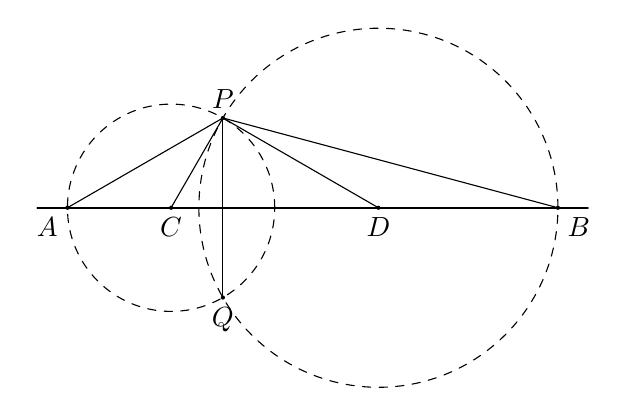
\begin{tikzpicture}[scale=0.38, line cap=round, line join=round]
  \pgfmathsetmacro{\sqt}{sqrt(3)}
  \pgfmathsetmacro{\Lseg}{6+6*\sqt}
  \pgfmathsetmacro{\Lext}{\Lseg+1}
  \pgfmathsetmacro{\cxx}{2*\sqt}
  \pgfmathsetmacro{\dxx}{6*\sqt}
  \pgfmathsetmacro{\pxx}{3*\sqt}
  \pgfmathsetmacro{\rCc}{2*\sqt}
  \coordinate (A) at (0,0);
  \coordinate (B) at (\Lseg,0);
  \coordinate (C) at (\cxx,0);
  \coordinate (D) at (\dxx,0);
  \coordinate (P) at (\pxx,3);
  \coordinate (Q) at (\pxx,-3);
  \draw[thick] (-1,0) -- (\Lext,0);
  \draw[dashed] (C) circle (\rCc);
  \draw[dashed] (D) circle (6);
  \draw (P) -- (Q);
  \draw (A) -- (P) -- (B);
  \draw (C) -- (P);
  \draw (D) -- (P);
  \fill (A) circle (2pt) node[below left] {$A$};
  \fill (B) circle (2pt) node[below right] {$B$};
  \fill (C) circle (2pt) node[below] {$C$};
  \fill (D) circle (2pt) node[below] {$D$};
  \fill (P) circle (2pt) node[above] {$P$};
  \fill (Q) circle (2pt) node[below] {$Q$};
\end{tikzpicture}
\end{center}

\textbf{Referencial.} Tomemos $A=(0,0)$ e $B=(L,0)$, com $L=m(\overline{AB})=6(1+\sqrt{3})$ cm e eixo $x$ sobre a reta $AB$. Como $C,D\in\overline{AB}$, temos $C=(c,0)$ e $D=(d,0)$ com $0\le c,d\le L$. Os raios são $r_C=m(\overline{CA})=c$ e $r_D=m(\overline{DB})=L-d$.

\textbf{Simetria.} $C\neq D$, pois circunferências concêntricas não se cortam em exatamente dois pontos. Como $C$ e $D$ são equidistantes de $P$ e de $Q$, a reta $CD=AB$ é a mediatriz de $\overline{PQ}$. Logo, a menos de reflexão em $AB$,
$$P=(p,h),\qquad Q=(p,-h),\qquad h>0,\qquad m(\overline{PQ})=2h.$$
Seja $x=m(\overline{AP})>0$. A hipótese $m(\overline{AP})=m(\overline{PQ})$ dá $h=\dfrac{x}{2}$.

\textbf{Passo 1.} Como $A=(0,0)$, $p^2+h^2=x^2$, logo $p^2=\dfrac{3x^2}{4}$.

\textbf{Passo 2 (circunferência $\mathcal{C}$).} $P\in\mathcal{C}$ significa $(p-c)^2+h^2=c^2$, isto é,
\begin{equation}
x^2=2pc.
\end{equation}
Aqui $c>0$, pois se $c=0$ a circunferência degenera no ponto $A\neq P$. Como $x>0$ e $c>0$, a igualdade (1) força $p>0$, e pelo Passo 1
\begin{equation}
p=\frac{\sqrt{3}}{2}\,x.
\end{equation}

\textbf{Passo 3 (condição sobre $\overline{BP}$).} Temos
$$m(\overline{BP})^2=(L-p)^2+h^2=L^2-2Lp+x^2=(2+\sqrt{3})\,x^2,$$
logo $2Lp=L^2-(1+\sqrt{3})\,x^2$. Substituindo (2):
$$(1+\sqrt{3})\,x^2+\sqrt{3}\,Lx-L^2=0\iff\big[(1+\sqrt{3})\,x-L\big](x+L)=0.$$
Como $x>0$ e $x+L>0$, resta $(1+\sqrt{3})\,x=L=6(1+\sqrt{3})$, ou seja,
$$m(\overline{AP})=m(\overline{PQ})=6\ \text{cm},\qquad h=3\ \text{cm},\qquad p=3\sqrt{3}\ \text{cm}.$$

\textbf{a) Raios.}

\emph{Raio de $\mathcal{C}$.} Por (1), $c=\dfrac{x^2}{2p}=\dfrac{36}{6\sqrt{3}}=2\sqrt{3}$ cm.

\emph{Raio de $\mathcal{D}$.} $m(\overline{DP})=m(\overline{DB})=r_D$ dá $(p-d)^2+h^2=(L-d)^2$, isto é, $(p-L)(p+L-2d)=-h^2$. Como $p<L$, isolando $d$:
$$r_D=L-d=\frac{(L-p)^2+h^2}{2(L-p)}=\frac{m(\overline{BP})^2}{2(L-p)}=\frac{36(2+\sqrt{3})}{2\cdot 3(2+\sqrt{3})}=6\ \text{cm},$$
usando $L-p=6+3\sqrt{3}=3(2+\sqrt{3})$. Então $d=6\sqrt{3}$ cm.

\emph{Verificação.} $0<2\sqrt{3}<6\sqrt{3}<L$, logo $C$ e $D$ estão em $\overline{AB}$. Além disso $m(\overline{CP})^2=3+9=12$ e $m(\overline{DP})^2=27+9=36$, como exigido. As circunferências são secantes, pois $|r_D-r_C|<CD=4\sqrt{3}<r_C+r_D$.

\textbf{Resposta a):} $r_{\mathcal{C}}=2\sqrt{3}\ \text{cm}\approx 3{,}46\ \text{cm}$ e $r_{\mathcal{D}}=6\ \text{cm}$.

\textbf{b) Área da região comum.} A corda $\overline{PQ}$ está na reta $x=x_0=3\sqrt{3}$. Os centros estão a $d_1=x_0-c=\sqrt{3}$ de $C$ e $d_2=d-x_0=3\sqrt{3}$ de $D$, em lados opostos da corda.

Sejam $\pi_{\mathcal{C}}(X)=|XC|^2-R_1^2$ e $\pi_{\mathcal{D}}(X)=|XD|^2-R_2^2$, com $R_1=2\sqrt{3}$ e $R_2=6$. A função $f=\pi_{\mathcal{C}}-\pi_{\mathcal{D}}=2(d-c)\,x+\text{const}$ é estritamente crescente em $x$ e se anula em $x=x_0$ (reta $PQ$). Logo:
\begin{itemize}
  \item se $x\ge x_0$ e $\pi_{\mathcal{C}}\le 0$, então $\pi_{\mathcal{D}}=\pi_{\mathcal{C}}-f\le 0$;
  \item se $x\le x_0$ e $\pi_{\mathcal{D}}\le 0$, então $\pi_{\mathcal{C}}=\pi_{\mathcal{D}}+f\le 0$.
\end{itemize}
Assim, a região comum é a união de dois segmentos circulares: o do disco $\mathcal{C}$ com $x\ge x_0$ e o do disco $\mathcal{D}$ com $x\le x_0$, que só se tocam na corda (área nula).

Os ângulos centrais são dados por $\cos\dfrac{\theta_1}{2}=\dfrac{d_1}{R_1}=\dfrac12$ e $\cos\dfrac{\theta_2}{2}=\dfrac{d_2}{R_2}=\dfrac{\sqrt{3}}{2}$, ou seja, $\theta_1=\dfrac{2\pi}{3}$ e $\theta_2=\dfrac{\pi}{3}$. Como cada centro está do outro lado da corda, ambos os segmentos são os menores. Usando $[\text{segmento}]=\dfrac{R^2}{2}(\theta-\operatorname{sen}\theta)$:
$$[S_1]=\frac{12}{2}\Big(\frac{2\pi}{3}-\frac{\sqrt{3}}{2}\Big)=4\pi-3\sqrt{3},\qquad [S_2]=\frac{36}{2}\Big(\frac{\pi}{3}-\frac{\sqrt{3}}{2}\Big)=6\pi-9\sqrt{3}.$$
Logo
$$[\text{região comum}]=10\pi-12\sqrt{3}\ \ \mathrm{cm}^2.$$

\emph{Conferência.} A região é o setor de $\mathcal{C}$ ($2\pi/3$) mais o setor de $\mathcal{D}$ ($\pi/3$), menos o quadrilátero $CPDQ$, cuja área é $\dfrac{CD\cdot PQ}{2}=\dfrac{4\sqrt{3}\cdot 6}{2}=12\sqrt{3}$ (diagonais perpendiculares). Obtemos $4\pi+6\pi-12\sqrt{3}$, o mesmo resultado. Numericamente, $10\pi-12\sqrt{3}\approx 10{,}63\ \mathrm{cm}^2$, valor menor que a área do disco $\mathcal{C}$, $12\pi\approx 37{,}7\ \mathrm{cm}^2$.

\textbf{Resposta b):} $(10\pi-12\sqrt{3})\ \mathrm{cm}^2\approx 10{,}63\ \mathrm{cm}^2$.

\noindent ANSWER: a) $r_{\mathcal{C}}=2\sqrt{3}\ \mathrm{cm}\approx 3{,}46\ \mathrm{cm}$ e $r_{\mathcal{D}}=6\ \mathrm{cm}$; b) $(10\pi-12\sqrt{3})\ \mathrm{cm}^2\approx 10{,}63\ \mathrm{cm}^2$
%
\newpage%
\section*{Apêndice: parecer do avaliador}%
\subsection*{Questão 1: nota 8,5 (não aprovada, rodada 3 de 3)}%
\textbf{Resposta da resolução às cegas do avaliador:} Resposta: 231 pontos com coordenadas inteiras no sólido fechado (129 no interior + 102 na superfície). Não é múltipla escolha. O sólido é \{(x,y,z) $\in$ $\mathbb{R}$$^3$ : |x|+|y|+|z| $\leq$ 5\}, e a contagem é feita sobre $\mathbb{Z}$$^3$.\par %
Resposta final 231 (129 no interior + 102 na superfície) está correta e coincide com a referência. Conferi por força bruta em Python sobre {[}{-}5,5{]}$^3$: interior (g$\leq$4) = 129, superfície (g=5) = 102, total 231. N\_k = 4k$^2$+2 para k$\geq$1 e N\_0 = 1 conferem para k=0..5. A fórmula fechada (2n+1)(2n$^2$+2n+3)/3 confere com contagem direta para n=0..6, e a identidade do item 6 vale. O volume 500/3 também confere. Pontos fortes: identificação do octaedro pelo argumento de antípodas (com a aresta 5$\surd$2 verificada), prova de K = S nos dois sentidos com pesos explícitos e não negativos, separação interior/superfície por perturbação $\varepsilon$, contagem por níveis disjuntos, verificação independente por tipos de coordenadas com sinais 2\^{}(não nulos) e fórmula fechada. Armadilhas tratadas: origem contada, sinais e permutações, aresta não tomada como 5, sólido fechado (interior + superfície), instrução 8 (expressões resolvidas até o número final). Não há erro matemático. A nota 8.5 (e não 9) decorre de lacunas de justificativa em fatos padrão (colinearidade dos ápices, fecho convexo, fechamento de S), notação sobrecarregada e uma seção 7 dispensável com heurística não quantificada. Todas as lacunas são menores e corrigíveis com poucas linhas."%
\begin{itemize}%
\item%
{[}minor{]} Seção 1: 'PM=QM' não basta para concluir que M é ponto médio de PQ. Falta mostrar que P, M e Q são colineares (os ápices estão sobre a reta perpendicular à base pelo centro). A antipodalidade dos vértices é afirmada, não demonstrada. Deveria haver uma frase sobre o eixo da pirâmide regular ou sobre a simetria do octaedro.%
\item%
{[}minor{]} Seção 2: 'O sólido é o fecho convexo K' é assumido sem justificativa. Falta dizer que um poliedro convexo é o fecho convexo de seus vértices (ou que é a união de duas pirâmides, cada uma fecho convexo de seus vértices).%
\item%
{[}minor{]} Seção 3: a identificação 'superfície = \{g=5\}' usa implicitamente que S é fechado, de modo que $\partial$S = S \textbackslash{} int S. Isso não é dito. Falta uma frase sobre o fechamento de S (imagem inversa de {[}0,5{]} por função contínua).%
\item%
{[}minor{]} Seção 1: o argumento entre parênteses ('se algum par não contivesse nenhum... o que é impossível') é confuso. Bastava dizer que os três pontos estão em três pares distintos e que há exatamente três pares.%
\item%
{[}minor{]} Notação sobrecarregada: P é ápice (seção 1) e ponto genérico (seções 2--3); M é centro do quadrado (seção 1) e função M(m) (seção 4); A é vértice dado A\_1 e também vértice da base ABCD. Renomear para evitar confusão.%
\item%
{[}minor{]} Não há discussão explícita da não{-}sobreposição de faces, arestas e vértices na contagem da superfície. A decomposição por níveis N\_k evita a dupla contagem, mas o texto não diz isso. Uma frase resolveria.%
\item%
{[}minor{]} Seção 7 é ruído: 'unidades' não se aplica a uma contagem, e a afirmação de que a diferença $\approx$ 64 é 'plausível como contribuição dos pontos de fronteira' não é quantificada. Há 102 pontos de fronteira, e a conexão correta é via Ehrhart: L(n) = 4n$^3$/3 + 2n$^2$ + 8n/3 + 1, em que 2n$^2$ vem da fronteira. Ou remover a seção, ou substituí{-}la por essa identidade, que é verificável.%
\end{itemize}%
\subsection*{Questão 2: nota 9,0 (aprovada, rodada 1 de 1)}%
\textbf{Resposta da resolução às cegas do avaliador:} n = 15.\newline%
\newline%
Resumo: A = I + N, com N nilpotente (N$^3$ = 0). Assim A? = I + nN + C(n,2)N$^2$, e a entrada (1,3) de A? é a? = n(n+3)/2. A condição a? > 119 equivale a (n-14)(n+17) > 0, logo n > 14 para n $\in$ $\mathbb{N}$. Como a$_{1}$$_{4}$ = 119 (não supera 119) e a$_{1}$$_{5}$ = 135, o menor n é 15.\par %
Resposta final conferida: n = 15, igual à referência, e correta. Refiz no Python (inteiros, n = 1..30): a forma {[}{[}1,n,n(n+3)/2{]},{[}0,1,n{]},{[}0,0,1{]}{]} confere com A\^{}n, o primeiro n com entrada (1,3) > 119 é 15, e (A\^{}14)\_13 = 119 (não estritamente maior). A indução do candidato está completa: a base n = 1 dá a\_1 = 2, o passo calcula corretamente A\^{}n$\cdot$A (colunas (1,0,0), (1,1,0), (2,1,1)) e a identidade a\_n + n + 2 = (n+1)(n+4)/2 = a\_\{n+1\} vale. A equivalência a\_n > 119 ? (n-14)(n+17) > 0 é exata para todo n $\in$ $\mathbb{N}$, então a minimalidade vem direto, sem depender de monotonicidade (mais forte que a argumentação da referência). Armadilhas: desigualdade estrita tratada (a\_14 = 119 excluído); raiz -17 descartada; índice (1,3) usado; itens 8 atendido (14$\cdot$17/2 = 119 e 15$\cdot$18/2 = 135 escritos como inteiros). Os problemas são apenas menores: a checagem de ordem de grandeza é enganosa (n$^2$/2 sugeriria 16), e o fechamento da indução poderia ser mais explícito. Texto de nível de gabarito comentado, com nota 9 pelas falhas menores de redação."\}%
\begin{itemize}%
\item%
{[}minor{]} A checagem de 'ordem de grandeza' (a\_n $\approx$ n$^2$/2, n$^2$ $\approx$ 238, 'coerente com o resultado') é falsa como verificação. Com a aproximação n$^2$/2 > 119 obtém{-}se n > 15,4, o que apontaria para n = 16. Só há concordância com n = 15 ao incluir o termo linear 3n/2. Deve ser removida ou reescrita de modo a não sugerir uma confirmação que a aproximação não dá.%
\item%
{[}minor{]} A frase 'As entradas (1,2) e (2,3) de A\^{}\{n+1\} são n+1, logo a forma vale para n+1' não menciona explicitamente as demais entradas (zeros e uns). Elas aparecem nos itens de linha acima, mas o fechamento da indução poderia dizer que as demais entradas coincidem com a forma pelas contas das três linhas.%
\item%
{[}minor{]} A resposta usa a convenção $\mathbb{N}$ = \{1,2,...\}, coerente com o enunciado, mas não a explicita. A base da indução em n = 1 depende dela. Uma menção curta evitaria ambiguidade para quem lê com $\mathbb{N}$ incluindo 0.%
\end{itemize}%
\subsection*{Questão 3: nota 9,0 (aprovada, rodada 2 de 2)}%
\textbf{Resposta da resolução às cegas do avaliador:} Área de ABCD = 30 (unidades de área). Questão dissertativa, não há alternativas. Valores intermediários: X = (3, 5/2) é o centro do paralelogramo; A = (-2, 0); B = (0, 4); C = (8, 5); D = (6, 1). Diagonal AC ? r e BD ? s; {[}ABX{]} = 15/2; o inraio de ABX é $\surd$5/2, igual ao dado.\par %
Resposta final 30 confere com a referência e com minhas contas (fração, fórmula de Gauss, det(AB,AD)=-30, $\frac12$|AC$\times$BD|=30, sen $\theta$=4/5). Enunciado do PDF confirmado: r: 2y-x=2, s: x+2y=8, C=(8,5), ? com centro (1/2,5/2) e r$^2$=5/4. Todas as armadilhas da referência foram tratadas: X como centro (não vértice), uso de sen $\theta$ (r e s não são perpendiculares), atribuição AC?r e BD?s por C$\in$r e C?s, A=2X-C com justificativa, sinal de r, $\rho$=$\surd$5/2, consistência d(I,r)=d(I,s)=$\rho$, escolha de AB como segunda tangente com descarte de m=1/2, observação sobre troca de B e D (distância 35/(2$\surd$65)$\approx$2,17 confirmada), verificação de inscrita (não excírculo) por sinais, B$\neq$X, B?r, condições do paralelogramo e três conferências independentes. A resolução é completa e correta; os problemas são pequenas lacunas de justificativa e clareza, sem impacto no resultado. Nota 9: publicável como gabarito comentado após pequenos ajustes."%
\begin{itemize}%
\item%
{[}minor{]} A afirmação de que os quatro triângulos ABX, BCX, CDX, DAX têm a mesma área é justificada só por 'X é ponto médio das duas diagonais'. Falta o argumento: {[}ABX{]}={[}CBX{]}=$\frac12${[}ABC{]} porque X é ponto médio de AC (análogo com BD), ou a simetria central em X, que leva A?C e B?D. O passo é verdadeiro, mas não está demonstrado.%
\item%
{[}minor{]} Na verificação pelos triângulos, 'S = 4$\cdot${[}ABX{]} = 4$\cdot$$\frac12$$\cdot$15 = 30' usa o valor 15 sem que {[}ABX{]} = 15/2 seja escrito explicitamente. O leitor precisa recuperar det = -15 do Passo 6. Deveria constar {[}ABX{]} = $\frac12$|det(B-A, X-A)| = 15/2.%
\item%
{[}minor{]} O Passo 4 se intitula 'r e s tangenciam ?', mas mostra apenas d(I,r) = d(I,s) = $\rho$. Falta enunciar explicitamente que distância do centro à reta igual ao raio equivale a tangência.%
\item%
{[}minor{]} A determinação de B (Passo 5) usa a hipótese '? é inscrita' para afirmar que AB é tangente, e só depois o Passo 6 verifica a inscrição. A lógica está correta, mas a frase 'Como B foi forçado pela condição de tangência, esta é a única escolha possível' deveria ser explicitamente condicional: 'supondo ? inscrita, AB é tangente, logo AB é a segunda tangente por A; reciprocamente, o Passo 6 confirma'.%
\item%
{[}minor{]} Notação: o produto '$\times$' é usado para o determinante 2D sem definição, e a matriz do Passo 8 tem como colunas AB e AD sem o dizer. Uma linha de definição tornaria a verificação autocontida.%
\end{itemize}%
\subsection*{Questão 4: nota 9,0 (aprovada, rodada 1 de 1)}%
\textbf{Resposta da resolução às cegas do avaliador:} Área total vermelha = $\pi$($\alpha$$^2$ + 32$\alpha$ + 528) = $\pi${[}($\alpha$+16)$^2$ + 272{]}, para $\alpha$ > 0.\newline%
\newline%
Resumo: o disco central (raio $\alpha$) é vermelho e contribui com $\pi$$\alpha$$^2$. Os anéis vermelhos são os de índice par, A\_2, A\_4, ..., A\_32, num total de 16. Cada anel A\_k tem área $\pi$(2$\alpha$ + 2k - 1). Somando os 16 anéis vermelhos e acrescentando o disco central, obtém{-}se $\pi$($\alpha$$^2$ + 32$\alpha$ + 528). Não há alternativa de múltipla escolha.\par %
Resposta final correta e idêntica à da referência: S\_vermelho($\alpha$) = $\pi$($\alpha$$^2$ + 32$\alpha$ + 528) = $\pi${[}($\alpha$+16)$^2$ + 272{]}, para $\alpha$ > 0. Reli o enunciado no PDF (página 5, Questão 04) e confere com a transcrição. Conferi as contas com python3 usando frações para $\alpha$ $\in$ \{1, 1/2, 3/7, 5, 10/3, 100\}: a área vermelha, a branca ($\pi$(32$\alpha$+496)) e a total ($\pi$($\alpha$+32)$^2$) batem em todos os casos, e a leitura alternativa de 34 circunferências dá o mesmo resultado. Todas as contas intermediárias do candidato conferem: A\_k = $\pi$(2$\alpha$+2k-1), A\_2 = 5$\pi$ em $\alpha$=1, $\Sigma$j = 136, S\_B = $\pi$(32$\alpha$+496), S\_V - S\_B = $\pi$($\alpha$$^2$+32) e diferença de cada par (A\_2j, A\_2j-1) igual a 2$\pi$. Armadilhas tratadas: disco central incluído ($\pi$$\alpha$$^2$), paridade das cores (vermelhos são os de índice par), 16 anéis vermelhos, área do anel como diferença de áreas, aritmética da soma, forma final expandida com $\pi$, verificação numérica em $\alpha$=1 (561$\pi$), e área branca e total separadas da resposta pedida. Os três problemas são menores: a leitura de \textbackslash{}"33 círculos\textbackslash{}" não é justificada nem a invariância é mencionada, uma frase sobre a soma está imprecisa, e $\alpha$>0 não é repetido no bloco ANSWER. Resolução publicável como gabarito comentado, com pequenos ajustes de redação."\}%
\begin{itemize}%
\item%
{[}minor{]} A leitura de "33 círculos" é apenas declarada ("contando o central"), sem justificativa no texto e sem mencionar a leitura alternativa (34 circunferências, isto é, 33 anéis além do central). A resposta é invariante nessa leitura, pois os anéis vermelhos continuam sendo A\_2,...,A\_32 e o 33º anel tem índice ímpar (branco). Deveria haver uma frase dizendo isso, porque o enunciado admite essa ambiguidade. Verificado em python: para $\alpha$=1, 7/3 e 50, as duas leituras dão o mesmo valor vermelho.%
\item%
{[}minor{]} Na seção de área vermelha, a frase "o termo 2$\alpha$-1 é somado 16 vezes" descreve mal a separação da soma. O termo é 2$\alpha$+4j-1, e o correto seria $\Sigma$(2$\alpha$-1) + 4$\Sigma$j = 16(2$\alpha$-1) + 4$\cdot$136. O resultado 32$\alpha$+528 está certo, mas a justificativa escrita está imprecisa.%
\item%
{[}minor{]} A restrição $\alpha$>0 aparece apenas no início ("Seja $\alpha$>0 o raio...") e não é repetida no bloco ANSWER. Também não há menção explícita de que a fórmula polinomial vale para qualquer $\alpha$ real positivo, inclusive não inteiro. A dedução é geral, então o problema é só de acabamento.%
\end{itemize}%
\subsection*{Questão 5: nota 9,0 (aprovada, rodada 2 de 2)}%
\textbf{Resposta da resolução às cegas do avaliador:} Razão pedida: V(esfera maior) / {[}4$\cdot$V(esfera menor){]} = (22 + 9$\surd$6)/16 $\approx$ 2,75.\newline%
\newline%
Passos{-}chave: aresta do tetraedro dos centros = 2r; circunraio do tetraedro regular = a$\surd$6/4 = r$\surd$6/2; raio da esfera maior R = r$\surd$6/2 + r = r(2+$\surd$6)/2; R$^3$/r$^3$ = (22+9$\surd$6)/4; razão = R$^3$/(4r$^3$) = (22+9$\surd$6)/16.\newline%
\newline%
Questão dissertativa (não há múltipla escolha). Resultado independente de r.\par %
Resposta final correta: (22+9$\surd$6)/16 $\approx$ 2,7528. Confirmei pelo enunciado original (página 6 da prova; a transcrição é fiel), por expansão algébrica exata e por cálculo numérico com python. Comparação item a item com a referência: aresta = 2r (igual); circunraio = r$\surd$6/2 (igual); R = r(2+$\surd$6)/2 (igual); razão = R$^3$/(4r$^3$) (igual); (2+$\surd$6)$^3$ = 44+18$\surd$6 (igual); resultado final (22+9$\surd$6)/16 (igual). Não há divergência. A resolução trata todas as armadilhas da lista: soma dos quatro volumes menores, ordem da razão (maior/soma), aresta 2r com argumento de tangência externa, circunraio a$\surd$6/4, tangência interna R = d + r, unicidade do circuncentro com argumento linear correto, expansão completa com a divisão por 4 explícita, e ausência de r no resultado. Os problemas são de clareza e de redação, não de conteúdo: a passagem de congruência no Passo 3, a verificação circular do item de 36\%, e a justificativa breve da não coplanaridade e da consistência da configuração. Nota 9: a resolução é publicável como gabarito comentado após os ajustes listados."%
\begin{itemize}%
\item%
{[}minor{]} Passo 3: a passagem 'Como dois tetraedros regulares de mesma aresta são congruentes, o centro O é o baricentro do tetraedro C1C2C3C4' é compressa. Não diz explicitamente que a isometria leva o circuncentro do modelo (a origem) ao circuncentro de C1\ldots{}C4, que é O pelo Passo 2, nem que isometrias preservam o baricentro. A conclusão está certa, mas a cadeia precisa ser escrita. Correção: explicitar essa cadeia, ou afirmar diretamente que num tetraedro regular o circuncentro coincide com o baricentro e o circunraio é a$\surd$6/4, usando a verificação por coordenadas só como comprovação.%
\item%
{[}minor{]} Verificação, segundo item: 'a razão 2,75 ... menores ocupam 1/2,75 $\approx$ 36\% ... valor que coincide com 4(r/R)$^3$ $\approx$ 0,363' não é verificação independente. 1/2,75 = 4(r/R)$^3$ é a mesma conta invertida. Correção: remover esse item ou reformulá{-}lo como simples reescrita; a verificação independente válida é a da altura/baricentro (3/4$\cdot$h), que o candidato já fez no item seguinte.%
\item%
{[}minor{]} Passo 2: a independência linear de C\_k - C\_1 é deduzida de 'os vértices não são coplanares', mas essa não coplanaridade não é justificada (decorre de o tetraedro ser não degenerado, aresta a = 2r > 0). Correção: acrescentar uma frase dizendo que o tetraedro regular é não degenerado, logo seus vértices não são coplanares.%
\item%
{[}minor{]} Consistência da configuração (menores contidas na maior e com interiores disjuntos) é afirmada na verificação, mas não argumentada. Ela segue de R = d + r (cada menor fica internamente tangente à maior) e de a = 2r (tangência externa entre menores, logo interiores disjuntos). Correção: uma frase conectando essas duas afirmações, como exige a lista de armadilhas sobre consistência da configuração.%
\end{itemize}%
\subsection*{Questão 6: nota 9,0 (aprovada, rodada 3 de 3)}%
\textbf{Resposta da resolução às cegas do avaliador:} Resposta de referência (enunciado impresso, lido literalmente):\newline%
\newline%
(a) det(AB) = 0. Vale para quaisquer $\alpha$\_j, porque A é estritamente triangular inferior (det A = 0).\newline%
\newline%
(b) tr(AB) = 0, constante e não dependente de n. O traço de AB é a soma de todas as entradas de A, que é igual à soma da coluna n de AB; a hipótese com j = n dá 0.\newline%
\newline%
(c) Nenhum valor. Para n = 5 o conjunto de ($\alpha$\_1, $\alpha$\_2, $\alpha$\_3, $\alpha$\_4) reais admissíveis é vazio. A hipótese é contraditória: as colunas n-1 e n de AB são iguais (a coluna n de A é nula), mas a hipótese exige somas 1 e 0.\newline%
\newline%
Ressalva: se a intenção for b\_ij = 1 para j $\leq$ i (triangular inferior), a resposta fica: $\alpha$\_1 = 0, $\alpha$\_3 = 0, $\alpha$\_2 $\in$ \{0, -1\}, $\alpha$\_4 $\in$ $\mathbb{R}$ arbitrário, com tr(AB) = 0 e det(AB) = 0. Recomenda{-}se confirmar a intenção com o gabarito oficial antes de penalizar (c).\par %
Respostas (enunciado impresso, conferido na página 7 do PDF): (a) det(AB)=0; (b) tr(AB)=0 (formal, pois a hipótese é impossível para n$\geq$2); (c) conjunto vazio. Coincidem com a referência e com a conta exata que fiz (n=2..7, 200 sorteios de $\alpha$): det=0 sempre, S\_\{n{-}1\}=S\_n sempre, e a hipótese exige 1 e 0. Na leitura alternativa (b\_ij=1 para j$\leq$i), a resolução também acerta: AB fica estritamente triangular inferior (det=tr=0), c\_j=1 para j=1..n-1, e para n=5 o conjunto é \{(0,0,0,t)\} ? \{(0,-1,0,t)\}, t$\in$$\mathbb{R}$ (conferido em grade racional). Armadilhas bem tratadas: coluna n de A nula; det(AB)=0 independente de $\alpha$ e de (H); convenção 0\^{}0=1 explícita; reais (1+$\alpha$+$\alpha$$^2$=($\alpha$+$\frac12$)$^2$+¾>0); $\alpha$\_4 livre; separação entre S\_k e c\_j; caso n=1; traço igual à soma das entradas de A (exemplo: 4, conferido). Não tratado: o argumento de c\_\{n{-}1\}=1 (ver issue 2). Texto claro, em formato de gabarito. Nota 9: publicável como gabarito comentado, com pequenos ajustes em (b) e na robustez da contradição. Observação: não consegui gravar memória sobre esta questão, porque o hook bloqueou escrita fora da pasta de trabalho e da prova."\}%
\begin{itemize}%
\item%
{[}minor{]} Item (b): o valor tr(AB)=0 sai de uma hipótese impossível para n$\geq$2 ($\sigma$\_n=0 e $\sigma$\_\{n{-}1\}=1 não podem ocorrer juntos). A resolução diz isso na ressalva, mas a resposta final (ANSWER) apresenta 'tr(AB)=0 para todo n' sem vincular o valor à contradição. Deveria apresentar primeiro a identidade tr(AB)=$\Sigma$ a\_ij=$\sigma$\_n, válida sem hipótese, e só depois concluir 0 sob (H), com a ressalva junto da resposta.%
\item%
{[}minor{]} Armadilha não tratada: a contradição pode ser vista sem usar a coluna n. Como c\_\{n{-}1\}=a\_\{n,n{-}1\}=$\alpha$\_\{n{-}1\}\^{}0=1 é forçado, a hipótese exigiria c\_\{n{-}1\}={-}1 (no n=5, c\_4 = $\sigma$\_4-$\sigma$\_3 = -1, mas c\_4 = a\_54 = 1). A resolução usa apenas $\sigma$\_n-$\sigma$\_\{n{-}1\}=c\_n=0, e isso depende de (H) valer também para j=n. Se (H) for lida só para j$\leq$n-1, o argumento apresentado não se aplica diretamente. Deveria acrescentar esse segundo argumento, que cobre as duas leituras.%
\item%
{[}minor{]} Passo 3 mostra apenas igualdade das somas das colunas n-1 e n de AB. Vale mais dizer que essas colunas são idênticas, pois a\_in=0 implica (AB)\_\{i,n{-}1\}=(AB)\_\{i,n\} para todo i. É uma formulação mais forte e mais clara do mesmo fato.%
\end{itemize}%
\subsection*{Questão 7: nota 9,0 (aprovada, rodada 1 de 1)}%
\textbf{Resposta da resolução às cegas do avaliador:} Raízes de p(x) em $\mathbb{C}$: x = -1, x = 1/2, x = 1 + 2i e x = 1 - 2i (todas simples).\newline%
\newline%
Polinômio obtido: p(x) = 2x$^{4}$ - 3x$^3$ + 7x$^2$ + 7x - 5 = (x + 1)(2x - 1)(x$^2$ - 2x + 5).\newline%
\newline%
Não se trata de questão de múltipla escolha. Desenvolvimento: p(x) = (x$^3$ - x + 4)(2x - 3) + (9x$^2$ - 4x + 7); as relações de Girard (soma -b/a = 3/2, produto (4b + 7)/a = -5/2) dão a = 2 e b = -3.\par %
A resposta final do candidato está correta e coincide com a da referência: raízes -1, 1/2, 1+2i e 1-2i, com p(x)=2x$^{4}$-3x$^3$+7x$^2$+7x-5=(x+1)(2x-1)(x$^2$-2x+5). Conferi o enunciado na página 8 do PDF e refiz todas as contas com aritmética exata: a=2 e b=-3 pelas relações de Girard (sinal + no produto, pois o grau é 4), a expansão dos coeficientes (9-a, 4a-b-4, 4b+7), o resto 9x$^2$-4x+7, as raízes racionais, a fatoração e as raízes 1$\pm$2i. Todas as conferências passaram. Das armadilhas da lista, o candidato evitou todas: não supôs p mônico, usou o sinal correto do produto, separou quociente linear e resto, usou as duas relações de Vieta, expandiu os termos com o resto corretamente, não recorreu às raízes do cúbico, não concluiu divisibilidade e deu as quatro raízes em $\mathbb{C}$. As falhas que restam são de rigor e apresentação, sem efeito no resultado. Nota 9: resolução que um professor publicaria como gabarito, com pequenos ajustes na justificativa da fatoração e na exibição de algumas contas numéricas.%
\begin{itemize}%
\item%
{[}minor{]} Passo 5: a afirmação "(x+1)(2x-1)=2x$^2$+x-1 divide p(x)" segue apenas de p(-1)=0 e p(1/2)=0, sem justificativa (teorema do fator para cada fator linear e não associação dos fatores, ou divisão explícita). A verificação por expansão no mesmo passo sustenta a identidade, então o erro é de rigor no encadeamento, não de conteúdo. Corrigir: citar o teorema do fator e dizer que o produto de fatores lineares distintos divide p, ou apresentar a divisão e o quociente x$^2$-2x+5.%
\item%
{[}minor{]} Passo 5: p(1/2)=1/8-3/8+7/4+7/2-5=0 é escrito sem passos intermediários. O enunciado do próprio caderno (instrução 8) exige que expressões numéricas sejam resolvidas integralmente. Corrigir: mostrar a redução, por exemplo 1/8-3/8+14/8+28/8-40/8=0.%
\item%
{[}minor{]} Passo 1: o fato de que o coeficiente líder de p é a (portanto c4=a) fica implícito. Só aparece na expansão do Passo 2 e no uso de c4 no Passo 3. Corrigir: uma frase dizendo que o coeficiente líder de p é a.%
\item%
{[}minor{]} Passo 3: as relações de Girard são enunciadas sem dizer que as raízes são contadas com multiplicidade em $\mathbb{C}$. Aqui não faz diferença, pois as raízes são simples, mas o enunciado geral fica incompleto. Corrigir: acrescentar "com raízes contadas com multiplicidade em $\mathbb{C}$".%
\item%
{[}minor{]} Armadilhas não comentadas explicitamente: a resolução não diz por que são necessárias duas relações de Vieta (a família de candidatos tem dois parâmetros), não diz que a não foi suposto igual a 1 e não observa que a hipótese de coeficientes reais não é necessária para determinar p. Não há erro nisso, mas um comentário breve deixaria a resolução no nível de gabarito comentado.%
\end{itemize}%
\subsection*{Questão 8: nota 9,0 (aprovada, rodada 1 de 1)}%
\textbf{Resposta da resolução às cegas do avaliador:} Resposta final: 784 sequências estritamente crescentes (a < b < c) de três números naturais ($\mathbb{N}$ = \{1, 2, 3, \ldots{}\}) com a + b + c = 100.\newline%
\newline%
Verificações: (i) soma $\Sigma$\_\{a=1\}\^{}\{32\} ?(99 - 3a)/2? = 784; (ii) round((100 - 3)$^2$/12) = round(9409/12) = 784; (iii) 833 partições não estritas - 49 com duas partes iguais = 784; (iv) força bruta = 784.\par %
Resposta final do candidato: 784. Minha resolução de referência também dá 784, então coincidem. Conferi por força bruta em Python: com $\mathbb{N}$ = \{1,2,3,\ldots{}\} o total é 784; se o zero fosse admitido, daria 833 (49 sequências extras com a=0). Verifiquei também a transformação x=a-1, y=b-a-1, z=c-b-1 (bijeção com N$_{0}$$^3$, 3x+2y+z=94), a soma $\Sigma$(48-3k)+$\Sigma$(46-3k)=408+376=784, e a contagem de soluções de 3x+2y+z=94, que dá 784.\newline%
\newline%
A resolução principal (Passos 1--3) é completa e rigorosa: a substituição que elimina as desigualdades está correta, a faixa x $\leq$ 31 está justificada, a separação em pares e ímpares cobre x=0..31 exatamente uma vez e os termos conferem. As três conferências independentes também estão corretas, mas são apresentadas com menos rigor do que a parte principal (fórmula citada sem justificativa, aproximação decimal contra a instrução 8, PA afirmada com reticências).\newline%
\newline%
Armadilhas da referência: todas tratadas. $\mathbb{N}$ começando em 1 com a observação do caso com zero (833); estritamente crescente com b $\geq$ a+1 e c $\geq$ b+1; sem multiplicar por 3!, com justificativa; 4704/6 tratado corretamente (não C(99,2)/6); limite a $\leq$ 32; desigualdades viram $\geq$ 0 nas novas variáveis; piso com paridade; fórmula (n-3)$^2$/12 usada no lugar certo; 3 ? 100 verificado explicitamente; expressões finais inteiras, exceto a aproximação da conferência 2.\newline%
\newline%
Nota 9: a resolução seria publicável como gabarito comentado. Os problemas são de apresentação nas conferências, não na resposta nem na prova principal.%
\begin{itemize}%
\item%
{[}minor{]} Conferência 2 enuncia a 'fórmula conhecida' round((n-3)$^2$/12) para partições em três partes distintas sem demonstração nem referência. O resultado é verdadeiro (a força bruta dá 784 para n=100), mas é uma afirmação geral não justificada. Deveria ser marcada explicitamente como resultado conhecido e usada só como conferência, ou ser substituída por uma verificação própria.%
\item%
{[}minor{]} Conferência 2 deixa 9409/12 como fração e chega a 784 por aproximação decimal ('$\approx$ 784,08'). Isso contraria a instrução 8 da prova (expressões numéricas devem ser resolvidas integralmente). Deveria escrever 9409 = 12$\cdot$784 + 1, logo 9409/12 = 784 + 1/12, cujo inteiro mais próximo é 784.%
\item%
{[}minor{]} Conferência 3 apresenta os valores de N(a) com reticências ('48, 46, 45, 43, \ldots{}, 3, 1') e afirma que o agrupamento a=2j+1 com a=2j+2 forma uma PA de 16 termos sem mostrar a conta. Faltam as expressões gerais: para a=2j+1, ?(99-a)/2? - a = 48 - 3j; para a=2j+2, vale 46 - 3j; a soma é 94 - 6j, com j=0..15. Também falta justificar 'positivos apenas para a $\leq$ 32': basta 97 $\geq$ 3a.%
\item%
{[}minor{]} Conferência 1 resume a inclusão{-}exclusão em 'dois empates implicam três iguais, logo não há interseções'. Está correto, mas condensado demais. Deveria dizer que as interseções duas a duas são todas \{a=b=c\}, que é vazio porque 3 ? 100, e por isso subtrair 3$\cdot$49 = 147 sem correção.%
\end{itemize}%
\subsection*{Questão 9: nota 9,0 (aprovada, rodada 1 de 1)}%
\textbf{Resposta da resolução às cegas do avaliador:} a) Há exatamente duas retas tangentes a H que passam por C = (0, -8): y = 2$\surd$6$\cdot$x - 8 (ou 2$\surd$6$\cdot$x - y - 8 = 0) e y = -2$\surd$6$\cdot$x - 8 (ou 2$\surd$6$\cdot$x + y + 8 = 0).\newline%
\newline%
b) Pontos de tangência: ($\surd$6, 4) para a reta y = 2$\surd$6$\cdot$x - 8, e (-$\surd$6, 4) para a reta y = -2$\surd$6$\cdot$x - 8.\newline%
\newline%
Base dos cálculos: c = 6, e = 3 $\Rightarrow$ a = 2, b$^2$ = 32, H: x$^2$/4 - y$^2$/32 = 1.\par %
Parecer sobre a Questão 09 (ITA 2026, 2ª fase).\newline%
\newline%
Conferência com o PDF original (página 10): o enunciado da transcrição confere (focos ($\pm$6,0), e = 3, C = (0,-8)).\newline%
\newline%
Resposta: correta e idêntica à referência nos dois itens.\newline%
a) y = 2$\surd$6$\cdot$x - 8 e y = -2$\surd$6$\cdot$x - 8 (equivalentes a 2$\surd$6$\cdot$x - y - 8 = 0 e 2$\surd$6$\cdot$x + y + 8 = 0).\newline%
b) ($\surd$6, 4) para a primeira reta e (-$\surd$6, 4) para a segunda.\newline%
\newline%
Verificação própria (python3): H: 8x$^2$ - y$^2$ = 32, com a = 2 e b$^2$ = 32. $\Delta$(m) = 128(24 - m$^2$), raiz dupla x = m/2, y = 4. Os pontos estão em H (1,000000000000). A inclinação da tangente em ($\surd$6,4) é 8x/y = 2$\surd$6 = m. Para m$^2$ = 8, a inclinação da tangente em (6/m, -2) é -3m $\neq$ m, então essas retas não são tangentes. A reta x = 0 não tem interseção real com H. A polar de C é y = 4 e corta H em x$^2$ = 6. A fórmula k$^2$ = a$^2$m$^2$ - b$^2$ com k = -8 dá m$^2$ = 24.\newline%
\newline%
Armadilhas: todas tratadas. e = c/a e a = 2; orientação x$^2$/4 - y$^2$/32 = 1; x = 0 excluída com justificativa; retas paralelas às assíntotas excluídas por um argumento de derivada, mais forte que a referência, que só observa 'um ponto comum não basta'; $\Delta$ com coeficiente líder não nulo (m$^2$ $\neq$ 8 tratado em caso separado); pareamento correto de sinais entre inclinação e ponto; polar com o sinal certo; 2$\surd$6 simplificado; pontos verificados em H.\newline%
\newline%
Não há divergência com a referência. A resolução é um gabarito sólido. Os problemas listados são menores: uma frase de simetria factualmente incorreta (C está sobre o eixo y, e não é 'simétrico' a H), uma definição de tangência circular, duas afirmações sem justificativa (a equivalência $\Delta$=0 $\Leftrightarrow$ tangente e a desigualdade |m| > b/a), um passo algébrico omitido e a falta da conclusão explícita de que há exatamente duas tangentes. Nenhum afeta a correção. Por isso a nota é 9: no limiar de gabarito publicável, subiria com as correções listadas.%
\begin{itemize}%
\item%
{[}minor{]} Na 'Simetria' do Passo 5 está escrito que 'H e C são simétricos em relação ao eixo y'. Isso está errado: H é simétrica em relação ao eixo y, e C = (0,{-}8) pertence a esse eixo, ou seja, é fixo pela reflexão. O argumento correto é que x ? {-}x leva o conjunto de tangentes por C em si mesmo, trocando m por {-}m e ($\surd$6,4) por ({-}$\surd$6,4). Corrigir a frase.%
\item%
{[}minor{]} No Passo 3, a definição de tangência é circular ('tem um único ponto comum com H e esse contato é de tangência'). Deveria definir tangência pela direção da reta igual à do gradiente no ponto de contato, ou pelo critério de um único ponto comum com reta não paralela a assíntota, enunciado de forma explícita.%
\item%
{[}minor{]} Para m$^2$ $\neq$ 8, a equivalência 'tangente $\Leftrightarrow$ $\Delta$=0' é afirmada sem justificativa. A direção '$\Delta$=0 $\Rightarrow$ tangente' fica implicitamente verificada pela derivada no Passo 5, mas a direção 'tangente $\Rightarrow$ $\Delta$=0' depende do fato de que uma tangente não paralela a assíntota tem um único ponto comum com H. Esse fato deveria ser citado ou provado em uma linha.%
\item%
{[}minor{]} A conta 'x = -16m/(2(8-m$^2$)) = m/2' pula a substituição de m$^2$ = 24, que dá 8-m$^2$ = -16 e -16m/(-32) = m/2. A instrução 8 da prova exige expressões numéricas resolvidas integralmente, então esse passo deveria aparecer explicitamente.%
\item%
{[}minor{]} A afirmação '|m| > b/a, como deve ser para tangentes que partem de C' é uma propriedade geral das tangentes não verticais de H (decorre de k$^2$ = a$^2$m$^2$ - b$^2$ $\geq$ 0). Está apresentada como conferência sem demonstração e sem ser ligada ao caso. Ou se demonstra em uma linha (com k = -8 dá m$^2$ = 24 > 8), ou se remove.%
\item%
{[}minor{]} A solução lista as duas retas, mas não conclui explicitamente 'há exatamente duas tangentes'. Essa conclusão de exaustividade decorre da análise (vertical excluída, m$^2$ = 8 excluída, $\Delta$=0 dá exatamente dois valores), e a polar y=4 cortando H em dois pontos a confirma. Vale escrever a frase final com esse argumento.%
\end{itemize}%
\subsection*{Questão 10: nota 9,0 (aprovada, rodada 1 de 1)}%
\textbf{Resposta da resolução às cegas do avaliador:} (a) Raio da circunferência de centro C: r\_C = 2$\surd$3 cm. Raio da circunferência de centro D: r\_D = 6 cm. Dados auxiliares: m(AP) = m(PQ) = 6 cm; m(AB) = 6(1+$\surd$3) cm; C = 2$\surd$3 cm e D = 6$\surd$3 cm medidos a partir de A, ambos dentro do segmento AB.\newline%
\newline%
(b) Área da região comum ao interior das duas circunferências: (10$\pi$ - 12$\surd$3) cm$^2$ $\approx$ 10,63 cm$^2$.\par %
Parecer sobre a Questão 10. As respostas finais coincidem com a referência e estão corretas (verificado com Python e integração numérica): (a) r\_C = 2$\surd$3 cm e r\_D = 6 cm; (b) área da região comum = 10$\pi$ - 12$\surd$3 cm$^2$ $\approx$ 10,63 cm$^2$. A prova usa um referencial de coordenadas com P = (p, h) e Q = (p, -h). A condição m(AP) = m(PQ) dá h = x/2. A condição sobre C dá x$^2$ = 2pc, e p > 0 vem de c > 0. A quadrática (1+$\surd$3)x$^2$ + $\surd$3Lx - L$^2$ = 0 é fatorada corretamente como {[}(1+$\surd$3)x - L{]}(x+L) = 0, com a raiz espúria -L rejeitada. A determinação de D é feita sem erro e o raio r\_D = m(BP)$^2$/(2(L-p)) está correto. A parte (b) é rigorosa: a função f = $\pi$\_C - $\pi$\_D é linear, nula na corda, e a lente é dividida nos dois segmentos corretos, com ângulos centrais 2$\pi$/3 e $\pi$/3. A verificação final de secância e de posição dos centros está feita. Problemas restantes, todos menores: o ramo $\alpha$ = 150$^\circ$ é eliminado sem ser nomeado nem justificado com a hipótese C$\in$AB; a verificação não recalcula a condição de BP; e há pequenas lacunas de exposição (expansão da equação (1), monotonicidade de f que exige d > c, justificativa da conferência por quadrilátero, redação da simetria). Nota 9: resolução correta, rigorosa e publicável como gabarito comentado após pequenos ajustes de exposição.%
\begin{itemize}%
\item%
{[}minor{]} Ramo espúrio $\alpha$ = 150$^\circ$ (p < 0) tratado apenas implicitamente. O Passo 2 elimina p<0 via 'c>0', mas a justificativa dada ('se c=0 a circunferência degenera') só exclui c=0. A exclusão de c<0 depende do 0$\leq$c da hipótese C$\in$AB, que não é citada nesse passo. Deveria: (i) citar C$\in$AB $\Rightarrow$ c$\geq$0; (ii) mostrar que p<0 daria c = x$^2$/(2p) = -x/$\surd$3 < 0; (iii) observar que esse ramo também satisfaz m(AP)=m(PQ) e a condição de BP, com x = L (raiz positiva da outra quadrática), e que só é descartado pela posição de C. Esta é a armadilha central do problema e merece menção explícita.%
\item%
{[}minor{]} Verificação final incompleta: confere CP, DP e a secância, mas não recalcula m(BP) = 6$\surd$(2+$\surd$3), que é a condição que fixou x. Deveria acrescentar: BP$^2$ = (6+3$\surd$3)$^2$ + 9 = 72 + 36$\surd$3 = 36(2+$\surd$3).%
\item%
{[}minor{]} No Passo 2, a equação (1) x$^2$ = 2pc aparece sem a linha intermediária: expandir (p-c)$^2$ + h$^2$ = c$^2$, usar p$^2$+h$^2$ = x$^2$ e obter p$^2$ - 2pc + h$^2$ = 0 $\Rightarrow$ x$^2$ = 2pc. Incluir para completude.%
\item%
{[}minor{]} Parte (b): a monotonicidade estrita de f = 2(d-c)x + const exige d > c, que só é conhecido após (a) e não é citado no argumento. Além disso, 'como cada centro está do outro lado da corda, ambos os segmentos são os menores' é ambíguo. O correto é: o segmento usado de cada círculo é o que fica do lado oposto ao seu centro, portanto é o menor (ângulo central < $\pi$). Deveria dizer isso explicitamente.%
\item%
{[}minor{]} Conferência de (b): afirma 'região = setor\_C + setor\_D - quadrilátero CPDQ' sem justificar. Faltaria observar que os triângulos CPQ e DPQ estão em semiplanos opostos de PQ, logo sua união é o quadrilátero CPDQ, cujas diagonais CD e PQ são perpendiculares e se cruzam no ponto médio de PQ, dando área CD$\cdot$PQ/2 = 12$\surd$3.%
\item%
{[}minor{]} Simetria: 'C e D são equidistantes de P e de Q' é imprecisa. O correto é que cada um de C e D está na mediatriz de PQ (CP = CQ e DP = DQ). Como C $\neq$ D, a reta CD = AB é essa mediatriz. Reformular a frase.%
\end{itemize}%
\end{document}